\chapter{Microbial population structure and genetic heterogeneity in a hypersaline environment}

\section{Abstract}

\section{Introduction}

The increasing number of microbial genomes being sequenced over the last few years, due to the drastic price reduction on the cost of sequencing a genome, has allow for comparisons among the genomes of closelry related microbial species and even more important strains from the same microbial species (REF). These comparisons have showed that even closely related strains of microorganisms, have enough differences in their genomic sequences that could explain their different functional behaivor (REF), and is a reflection of the different evolutionary histories of each strain (REF). This has been studied in detail specially in medical applications, where É. [Multiple studies and genomes, selective pressure].
In non-medical studies, a recent studie by (Science, shapiro), studied multiple Vibrio genomes, comparison, etcÉ.

With the development of community genomics approaches, we have knwo started to comprehend the level of genetic variation that can be found in natural microbial population (multiple REFs). In particular, the use of assembly-based approaches, allows us to reconstruct genomes (consensus o poulation genomes) from the members of the microbial community under study, and then using bioinformatic approaches, we can assest the level of genetic diversity that is present in a microbial population (REF). Most of the current studies have focus on very simple systems (REF, ISMEJ, enrichemnts) or only on a few members of the population under study (REF, Jill). In contrast, one of the studies that used a great amount of available data was based on metagenomic sequenecs obtained from the human microbiome, but in this case the genomes used were not necessary obtained from the same samples where the metagenomic sequences were obtaiend.
In this work, we used as a foundation the available information that was recovered from a assembly-based metagenomic study in the Lake Tyrreell hypersaline ecosystem, using the information as a reference, and then using deep-sequencing approaches, using Illumina sequencing, to assest and study the level of genetic variation that is present in a natural microbial community. Based on this information we can assest the level of genetic variation between populations, and also start to comprehend the effect of natural selection in these populations. (REFs, check microbiome paper).

we can observe the current status of the community, and ask questions later by sampling other times (establish a baseline for future studies).

\section{Material and Methods}

\subsection{Sample collection and sequencing}
Surface water samples from Lake Tyrrell were collected in 2007, at two different seasons, summer (January) and winder (August), with with two days of difference in each season (January 23 and 25, August 7 and 9). Each water sample was filtered directly into an Sterivex cartridge (Milipore, Bedford, MA, USA) (\SI{0.22}{\micro\meter}) using a peristaltic pump. For DNA extraction each Sterivex was processed according to the following protocol:
\begin{itemize}
\item Addition of Proteinase K to a final concentration of 0.5 mg/ml\textsuperscript{-1} and SDS to a final concentration of 1\%.
\item Incubation at 55\textsuperscript{o}C for 25 minutes, followed by incubation at 70\textsuperscript{o}C for 5 minutes.
\item Transfer of the lysate from the Sterivex, to a clean Eppendorf tube.
\item Nucleic acid extraction with two steps of phenol:chloroform extraction. 
\end{itemize}

For all four samples, the sequencing library construction was performed by the UC San Diego IGM Genomics Center. The four libraries were multiplexed and run on a single lane on an Illumina HiSeq machine, on high-throughput mode (2X100 PE reads).

After demultiplexing using the Illumina software, all the reads were processed using Nesoni 0.117 (http://www.vicbioinformatics.com/software.nesoni.shtml), to remove adapters, trim low quality positions and remove low quality reads from the datasets. For trimming a minimum quality score of 20 was used, and all reads shorter than 70 nucleotides (after trimming) were removed.

\subsection{Read mapping}

The trimmed reads were mapped against a set of habitat-specific genomes (Table \ref{GenomeTable} generated by the assembly of metagenomic information of the Lake Tyrrell microbial community \cite{Narasingarao:2012kp,Podell:2013kx,Podell:2013fp}. In addition, an archaeal isolate, \textit{Candidatus} Halobonum tyrrellensis \cite{Ugalde:2013hb}, obtained from samples collected in August of 2007, was also included in the analysis. Each sample was mapped independently to the set of reference genomes, using Bowtie 2.2.1 \cite{Langmead:2012jh} with the \textit{very-sensitive} alignment option, and adjusting the N-ceiling function to 0,0.01 to reduce the number of ambiguous characters present in the alignment. Several tools were used in the analysis of the resulting files, including SAMtools 0.1.19\cite{Li:2009ka}, BEDtools 2.17 \cite{Quinlan:2010km} and BCFtools 0.2.0 (http://samtools.github.io/bcftools/bcftools.html)

\subsection{Taxonomic classification}

The mapped and unmapped reads were classified using Phylosift 1.0.1 \cite{Darling:2014ej}, using the provided set of marker genes. This set included all of the January 2007 genomes assembled from the Lake Tyrrell community \cite{Narasingarao:2012kp,Podell:2013kx}, but did not included the newest one from the August 2007 community \cite{Podell:2013fp}.

\subsection{Variation analysis}

The mapped reads were processed using Picard Tools 1.99 (http://picard.sourceforge.net), and then GATK XXX (\cite{DePristo:2011fo} was used to realign indel regions to the reference genomes. The corrected files were processed with Freebayes v9.9.2-29-g9ed353c \cite{Garrison:2012wb} (ploidy:1, minimum base quality: 20, minimum mapping quality: 30). Quantification of the type of variations was done using SNPeff \cite{Cingolani:2012cz}, and custom Python scripts. 

Calculation of the pN/pS values was done using custom Python scripts (available in XXX), based on the approach used in Tai \textit{et al.} \cite{Tai:2011jo}. For each gene the pN/pS value was calculated as:

\begin{center}
\scalebox{1.6}{
\(
\frac{\text{pN}}{\text{pS}} = \frac{\frac{\text{Observed non synonymous mutations}}{\text{Number of non synonymous sites}}}{\frac{\text{Observed synonymous mutations}}{\text{Number of synonymous sites}}}
\)
}
\end{center}

\subsection{Computational resources and data availability}

All of the analysis were carried out using a large cluster instance (c3.8xlarge: 32 Intel Xeon E5-2680 v2 cores, 60 Gb RAM) on the elastic cloud computing resource at Amazon. Plotting and calculations were carried out using custom developed Python scripts. The majority of the code and preliminary analyses are available on a Github repository (XXX).

\begin{table}[!htdp]
\caption{List of the Lake Tyrrell habitat-specific genomes used for read mapping}
\begin{center}
\resizebox{\textwidth}{!}{%
\begin{tabularx}{\textwidth}{p{5cm}p{2cm}lp{2cm}p{1cm}}
\hline
\textbf{Genome name (abbrv)} & \textbf{Length} & \textbf{G+C pct} & \textbf{N scaffolds} & \textbf{Reference} \\
\hline
\textit{Haloquadratum walsbyi} J0HQW1 & 3,549,539 & 47 & 1 & \cite{Podell:2013kx} \\
\textit{Haloquadratum walsbyi} J0HQW2 & 3,475,501 & 49 & 1 & \cite{Podell:2013kx} \\
\textit{Haloquadratum} sp. J07HQX50 & 3,019,909 & 50 & 2 & \cite{Podell:2013kx} \\
\textit{Nanosalinarum} sp. J07AB56 & 1,215,802 & 56 & 3 & \cite{Narasingarao:2012kp} \\
\textit{Nanosalinarum} sp. J07AB43 & 1,277,157 & 43 & 7 & \cite{Narasingarao:2012kp} \\
\textit{Halonotius} sp. J07HN4 & 2,888,659 & 61 & 2 & \cite{Podell:2013kx} \\
\textit{Halonotius} sp. J07HN6 & 2,529,000 & 63 & 6 & \cite{Podell:2013kx} \\
uncultured archaeon sp. J07HX64 & 2,982,938 & 64 & 1 & \cite{Podell:2013kx} \\
uncultured archaeon sp. J07HX5 & 2,040,945 & 60 & 1 & \cite{Podell:2013kx} \\
\textit{Halobaculum} sp. J07HB67 & 2,649,547 & 67 & 3 & \cite{Podell:2013kx} \\
\textit{Halorubrum} sp. J07HR59 & 2,120,805 & 59 & 7 & \cite{Podell:2013kx} \\
\textit{Salinibacter} sp. J07SB67 & 1,931,021 & 67 & 443 & \cite{Podell:2013kx} \\
\textit{Halorubrum} sp. A07HR60 & 2,876,249 & 59 & 14 & \cite{Podell:2013fp} \\
\textit{Halonotius} sp. A07HN63 & 2,392,686 & 63 & 37 & \cite{Podell:2013fp} \\
\textit{Halorubrum} sp. A07HR67 & 2,890,468 & 67 & 16 & \cite{Podell:2013fp} \\
uncultured archaeon A07HB70 & 2,389,822 & 71 & 15 & \cite{Podell:2013fp} \\
\textit{Candidatus} Halobonum tyrellensis G22 & 3,675,087 & 70 & 72 & \cite{Ugalde:2013hb} \\
\hline

\end{tabularx}
}
\end{center}
\label{GenomeTable}
\end{table}


%\subsection{Simulated Illumina datasets}
%
%For each of the archaeal reference genomes (Table X), a set of simulated Illumina reads was generated using the sofware Grinder \cite{Angly:2012hm}. For each genome, the 
%(REF). The coverage for each genome was simulated at 50X, with paired-end reads of length 150 and an average insert size of 500. This reads were subsequently analyzed in the same manner as the sample dataset (mapping and SNP identification).

%\subsection{Assembly-based polymorphisms}
%
%The original assembly of the Lake Tyrrell metagenome dataset, was performed using Celera Assembler Version 5.4 \cite{Myers:2000wk}, as described in \cite{Narasingarao:2012kp, Podell:2013kx}. To generate a set of SNPs based on this assembly, the output of the assembly was processed with the AMOS package Version 2.0.8 \cite{Phillippy:2008if}, using the \textit{analyzeSNPs} module to generate a list of polymorphic sites within each scaffold of the assembled genomes from the January 2007 dataset (due to technical limitations, this procedure could not be applied to the August 2007 genomes). As some of the genomes were generated by combining Sanger and 454 reads \cite{Narasingarao:2012kp, Podell:2013kx}, only those positions that were supported by Sanger reads were considered in the analysis, discarding the 454 reads from the analysis. The reason behind this decision, is to allow a more stringent selection of polymorphisms, reducing the possibility of errors due to homopolymers. A position was considered in the SNP reference list if that position had a coverage of at least 4 reads (with a quality score of 20 or more) and the variant was supported by at least 3 reads. Processing of all the data was done using custom Python scripts and visualized in IPython \cite{Perez:2007wf} [Appendix?].
%
%To evaluate the effect of each SNP on the each genome, the program snpEff was used. This allowed the annotation of each SNP, into coding regions and also the type of modification and effect that the SNP could make on the amino acid sequence.

\clearpage
\section{Results and Discussion}

\subsection{Overview of the Illumina dataset for January and August of 2007}

Between 71-74\% of the original reads were retained after trimming and quality filtering (Table \ref{LibSequenceQC}). An approach to easily visualize the community composition and identify broad differences in population composition between samples, is to quantify the G+C content of the reads and plot the abundance by bins (usually of size 1\%) \cite{Podell:2013kx,Ghai:2012fb,Podell:2013fp}. Figure \ref{ReadsGCplot}, shows the differences between the four libraries, and highlights the previously assembled genomes from the Lake Tyrrell microbial community \cite{Narasingarao:2012kp,Podell:2013kx,Podell:2013fp}. The plot allows to identify the different populations present in the January versus the August libraries, in particular where the January community is dominated by organisms with lower G+C content, compared to the August community. This agrees with previous observations in the same microbial community \cite{Podell:2013fp}, where the main driver of these differences was suggested to be the ionic composition of the water column, in particular magnesium (Table \ref{LT_chemical}). Microorganisms like \textit{Haloquadratum} (J07HQW1, J07HQW2 and J07HQX50) are more dominant in the January samples, compared to the August samples. 

Another interesting observation that emerge from this G+C plot, is that the August samples have similar compositions based on the G+C content, while the January samples show differences. This could be possibly attributed to the differences in magnesium concentrations (Table \ref{LT_chemical}) between the two days in January, which could explain the increase in the \textit{Haloquadratum} populations on the January 25th sample, and in general of populations with a lower G+C content. Looking at possible explanations for this, we found on the weather records, that a storm occurred previous to the January 23th sampling, suggesting that the input of freshwater diluted the salt concentrations in the water column, reducing the magnesium concentration. After two days, due to water evaporation and other environmental factors, the magnesium concentration raised, explaining the difference that we see between the two days.



%Table, Summary libraries
\begin{table}[hbt]
  \caption{Summary of the Illumina HiSeq libraries for each of the four samples.}
  \begin{tabularx}{\textwidth}{L{2.2cm}R{2cm}R{3cm}R{3.2cm}R{2cm}}
  \hline
    \textbf{Library name} & \textbf{Total reads} & \textbf{Read-pairs after QC} & \textbf{Unpaired reads after QC} & \textbf{Total bases (Gb)} \\
    \hline 
    \textit{January 23} & 49,963,357 & 37,016,243 & 7,679,004 & 7,978.18\\
    \textit{January 25} & 39,400,015 & 29,444,267 & 5,894,815 & 6333.12 \\
    \textit{August 7} & 46,472,319 & 33,485,834 & 7,659,231 & 7266.38 \\
    \textit{August 9} & 40,256,946 & 28,843,346 & 6,812,171 & 6276.12 \\
  \end{tabularx}
  \label{LibSequenceQC}
\end{table}
%END

%Figure GC plot
\begin{figure}[!hbtp]
  \centering
  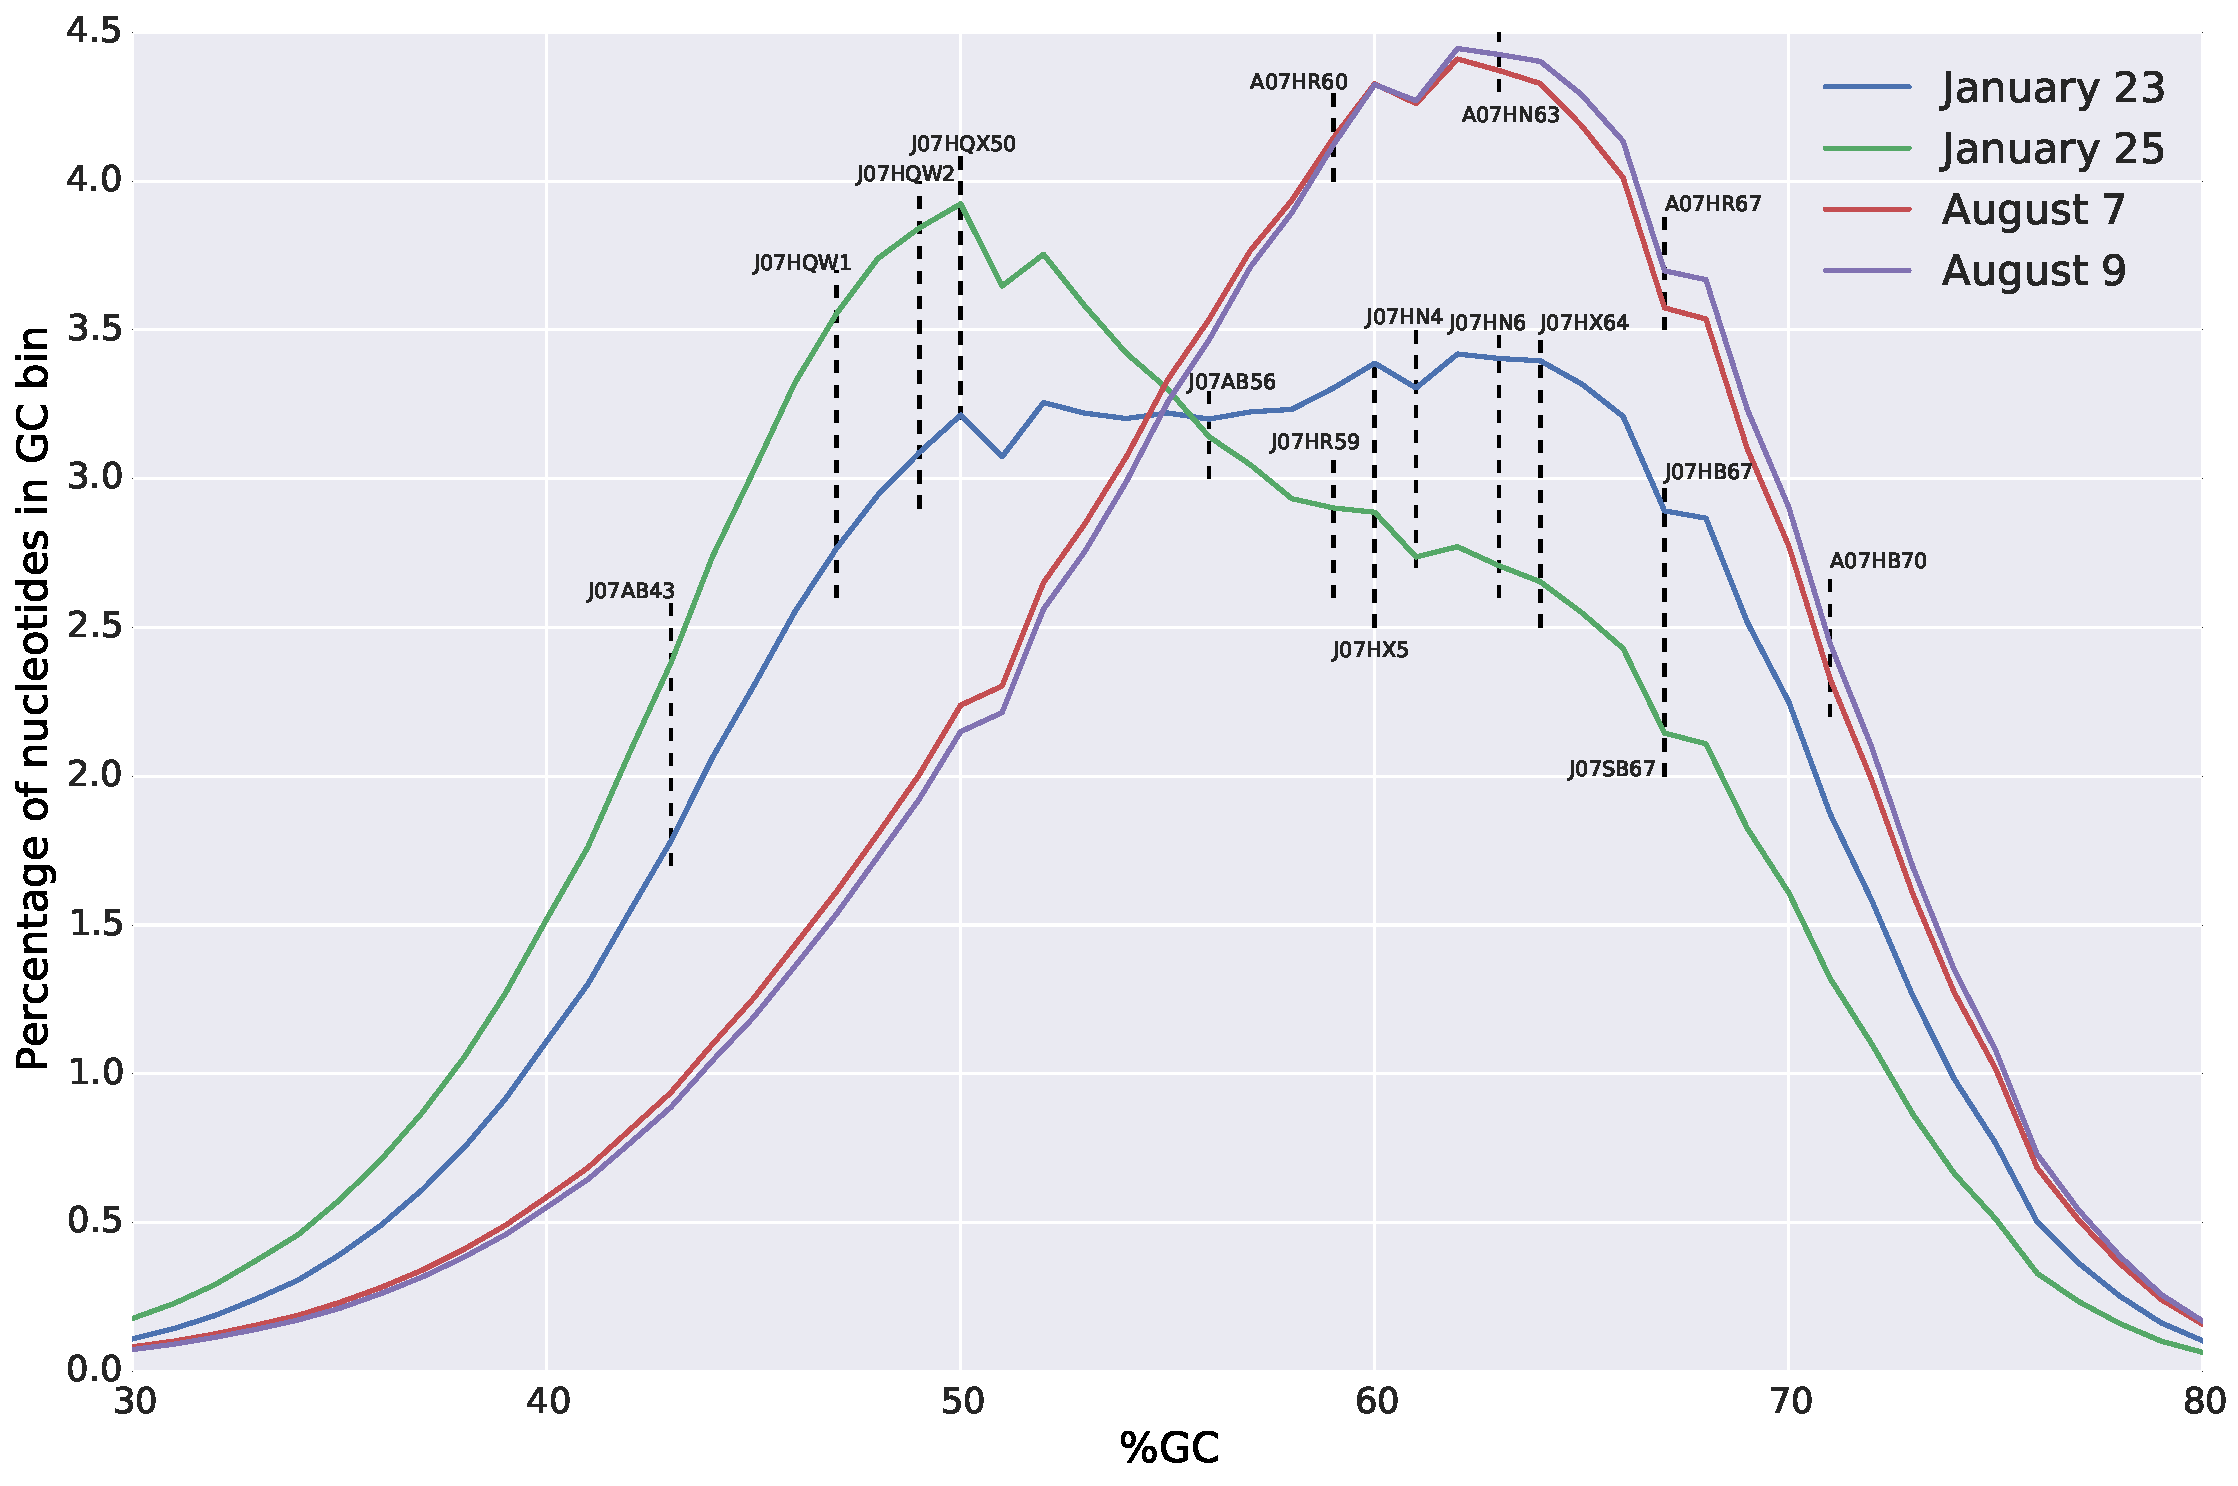
\includegraphics[width=\textwidth]{Chapter5/Figures/GC_content_HiSeqLibs.pdf}
  \caption{GC plot of libraries}
  \label{ReadsGCplot}
\end{figure}
%End of figure

%Table on a new page with facing caption
%\clearpage
\thispagestyle{facingcaption}
\begin{table}[h]
\captionsetup{labelformat=prev-page}
\caption{\textbf{Table \ref{LT_chemical}:} Physical and chemical composition of the Lake Tyrrell water samples. Concentrations are given in units of \si{\milli\mole\per\liter}}
\label{LT_chemical}
\end{table}
\clearpage

\begin{sidewaystable}[h]
\ContinuedFloat
\captionsetup{labelformat=empty}
\centering

\begin{tabular}{cccccccccc}

\textbf{Sample} & \textbf{Temp \si{\degreeCelsius}} & \textbf{Total ionic strength} & \textbf{Na} & \textbf{K} & \textbf{Mg} & \textbf{Ca} & \textbf{Cl} & \textbf{Cl} & \textbf{SO42} \\
\hline
\textit{Jan 23} & 21.6 & pH & 5,721 & 4,338 & 32 & 298 & 10 & 5,345 & 123.6 \\
\textit{Jan 25} & 27.9 & 7.09 & 5,950 & 4,163 & 43 & 419 & 11 & 5,291 & 170.5 \\
\textit{Aug 6} & 9.9 & 7.00 & 4,403 & 3,724 & 19 & 126 & 15 & 4,298 & 50 \\
\textit{Aug 8} & 11.5 & 7.01 & 4,060 & 3,557 & 18 & 117 & 14 & 3,830 & 47 \\

\end{tabular}
\end{sidewaystable}

%%%%End of table

%END OF SECTION
\clearpage
\subsection{Genome abundance and community structure, based on read mapping}

All of the reads that passed the quality filters were mapped against the set of reference genomes (Table \ref{GenomeTable}). The summary of this mapping (Table \ref{ReadRecruitmentGenome}), shows the difference in the number of reads that mapped to each genome. In both January samples, the \textit{Haloquadratum} J07HWQ1 and J07HWQ2 genomes, recruited the largest number of reads, which agrees with previous estimation of their abundance in the Lake Tyrrell community \cite{Podell:2013kx}. It is important to highlight that number of mapped reads to each genome, do not reflect the real abundance of each organism in the community. Given the strict criteria used for mapping, it is likely that we are missing information on some of these genomes (more on this later), and also several of these genomes represent closely related species, sharing the same DNA sequences. In addition, variations due to genome size and even genome copy number need to be taken in consideration. This explains, for example, why the \textit{Nanohaloarchaea} genomes (J07AB56 and J07AB43) do not recruit a large percentage of the reads, in contrast with their estimated high abundance in this community \cite{Podell:2013kx}. This stringent criteria, also explain why the genome of \textit{Candidatus} Halobonum tyrrellensis (G22), recruits a low number of reads from the dataset. This particular organisms, is an interesting situation, as it was isolated from surface waters collected in August of 2007, and by 16S showed to be similar to the \textit{Halobaculum} genomes assembled from the January and August samples (J07HB67 and A07HB70). Further analysis using the complete sequence, showed that it was a different population, and possibly a new Genus within the Haloarchaea \cite{Ugalde:2013hb}. This is a clear example on how in many situations, isolates from an environment are not representative of the most abundant members that can be found living in that environment.

A visualization of the numbers of mapped reads at different identity levels (Figure \ref{GenomeReadIdentity}), shows that for all the genomes (with the exception of G22), the majority of the reads mapped at a 100\% identity, and in none case was lower than 85\%. This reflects the stringency of the parameters used for mapping, and also allows to be confident that the reads are derived from that particular population. Looking more in detail to each of the individual genomes, these plots already show some information on the possible strain diversity present in each of the populations. In the case of the \textit{Haloquadratum} genomes, most of the reads mapped at identities of 95\% or higher, reflecting a low level of population heterogeneity among these populations. On the other extreme, in the case of the \textit{Salinibacter} populations, we can observe a range of identities going from 88\% and higher. 

Given the deep coverage of the community in this four libraries (an average of 4.3 billion nucleotides in each one), this dataset represent not only the most abundant members of the community, represented in the reference genomes used for mapping, but also allows access to less abundant organisms. To quickly evaluate the differences between the mapped and unmapped reads, we used a taxonomic classification approach to estimate difference between the mapped and unmapped reads on each dataset. For example, for the mapped reads in the January 23 dataset (Figure \ref{Jan23_Mapped}), as expected the majority of the mapped reads were classified as \textit{Haloquadratum}, followed by the \textit{Nanohaloarchaea}. In comparison, the unmapped reads for this library (Figure \ref{Jan23_Unmapped}), shows a diversity of groups, including a high percentage of Bacterial reads. These difference in taxonomic composition between the set of mapped and unmapped reads, can be visualize in a two-dimensional plot using an Edge principal component (EPCA) analysis \cite{Matsen:2011wn} derived from the Phylosift results. Plotting the first two components shows that based on the predicted taxonomic composition of the community, the reads separate between the mapped and unmapped groups, and in addition there is a separation by season in the case of the unmapped reads. For the mapped reads, we observe that the group separately from the unmapped, but due to technical problems, the data available is only for two of the libraries, one from each month. 

The taxonomic analysis suggests the presence of novel groups (not represented in the current set of genomes used for mapping) present in the community, and that with further analysis could be recovered. In the present work, I will focus only on the genomes and its mapped reads, as this genomes provide an already validated set of habitat-specific genomes that can be used for the analysis of diversity in this microbial community.

\begin{table}[ht!]
  \caption{Number of reads from each library, recruited to the Lake Tyrrell reference genomes}
  \begin{tabularx}{\textwidth}{L{2.2cm}R{2cm}R{3cm}R{3.2cm}R{2cm}}
  \hline
    \textbf{Genome} & \textbf{Jan 23} & \textbf{Jan 25} & \textbf{Aug 07} & \textbf{Aug 09} \\
    \hline
     \textit{J07HWQ1} & 9,712,976 & 10,347,084 & 1,802,421 & 1,385,337 \\
     \textit{J07HWQ2} & 7,311,175 & 9,428,490 & 1,628,137 & 1,301,141 \\
     \textit{J07HQX50} & 922,138 & 1,041,326 & 501,477 & 330,307 \\
     \textit{J07AB56} & 565,197 & 266,831 & 194,445 & 165,278 \\
     \textit{J07AB43} & 760,203 & 486,360 & 63,209 & 64295 \\
     \textit{J07HN4} & 2,149,204 & 2,249,692 & 1,306,287 & 1,089,673 \\
     \textit{J07HN6} & 592,818 & 831,367 & 1,027,472 & 911,341 \\
     \textit{J07HX64} & 4,167,113 & 1,819,023 & 1,202,103 & 1,144,206 \\
     \textit{J07HX5} & 2,106,559 & 1,382,371 & 673,972 & 539,843 \\
     \textit{J07HB67} & 1,124,816 & 1,128,191 & 125,973 & 84,643 \\
     \textit{J07HR59} & 839,856 & 310,496 & 2,105,598 & 1,693,772 \\
     \textit{A07HB70} & 550,429 & 277,030 & 1,970,106 & 1,866,967 \\
     \textit{A07HR67} & 563,043 & 270,602 & 2,166,129 & 1,680,150 \\
     \textit{A07HN63} & 547,808 & 786,856 & 1,126,032 & 1,003,322 \\
     \textit{A07HR60} & 2,126,700 & 758,549 & 5,405,933 & 4,362,857 \\
     \textit{G22} & 62,983 & 39,696 & 72,261 & 66,778 \\
     \textit{J07SB} & 797,957 & 211,306 & 737,471 & 673,630 \\     
  \textit{Unmapped} & 45,344,829 & 31,913,858 & 51,012,461 & 44,849,506 \\
  \end{tabularx}
  \label{ReadRecruitmentGenome}
\end{table}

%Figures for this section

%Figure, Genome Identity Plots
\begin{figure}[!hbtp]
  \centering
  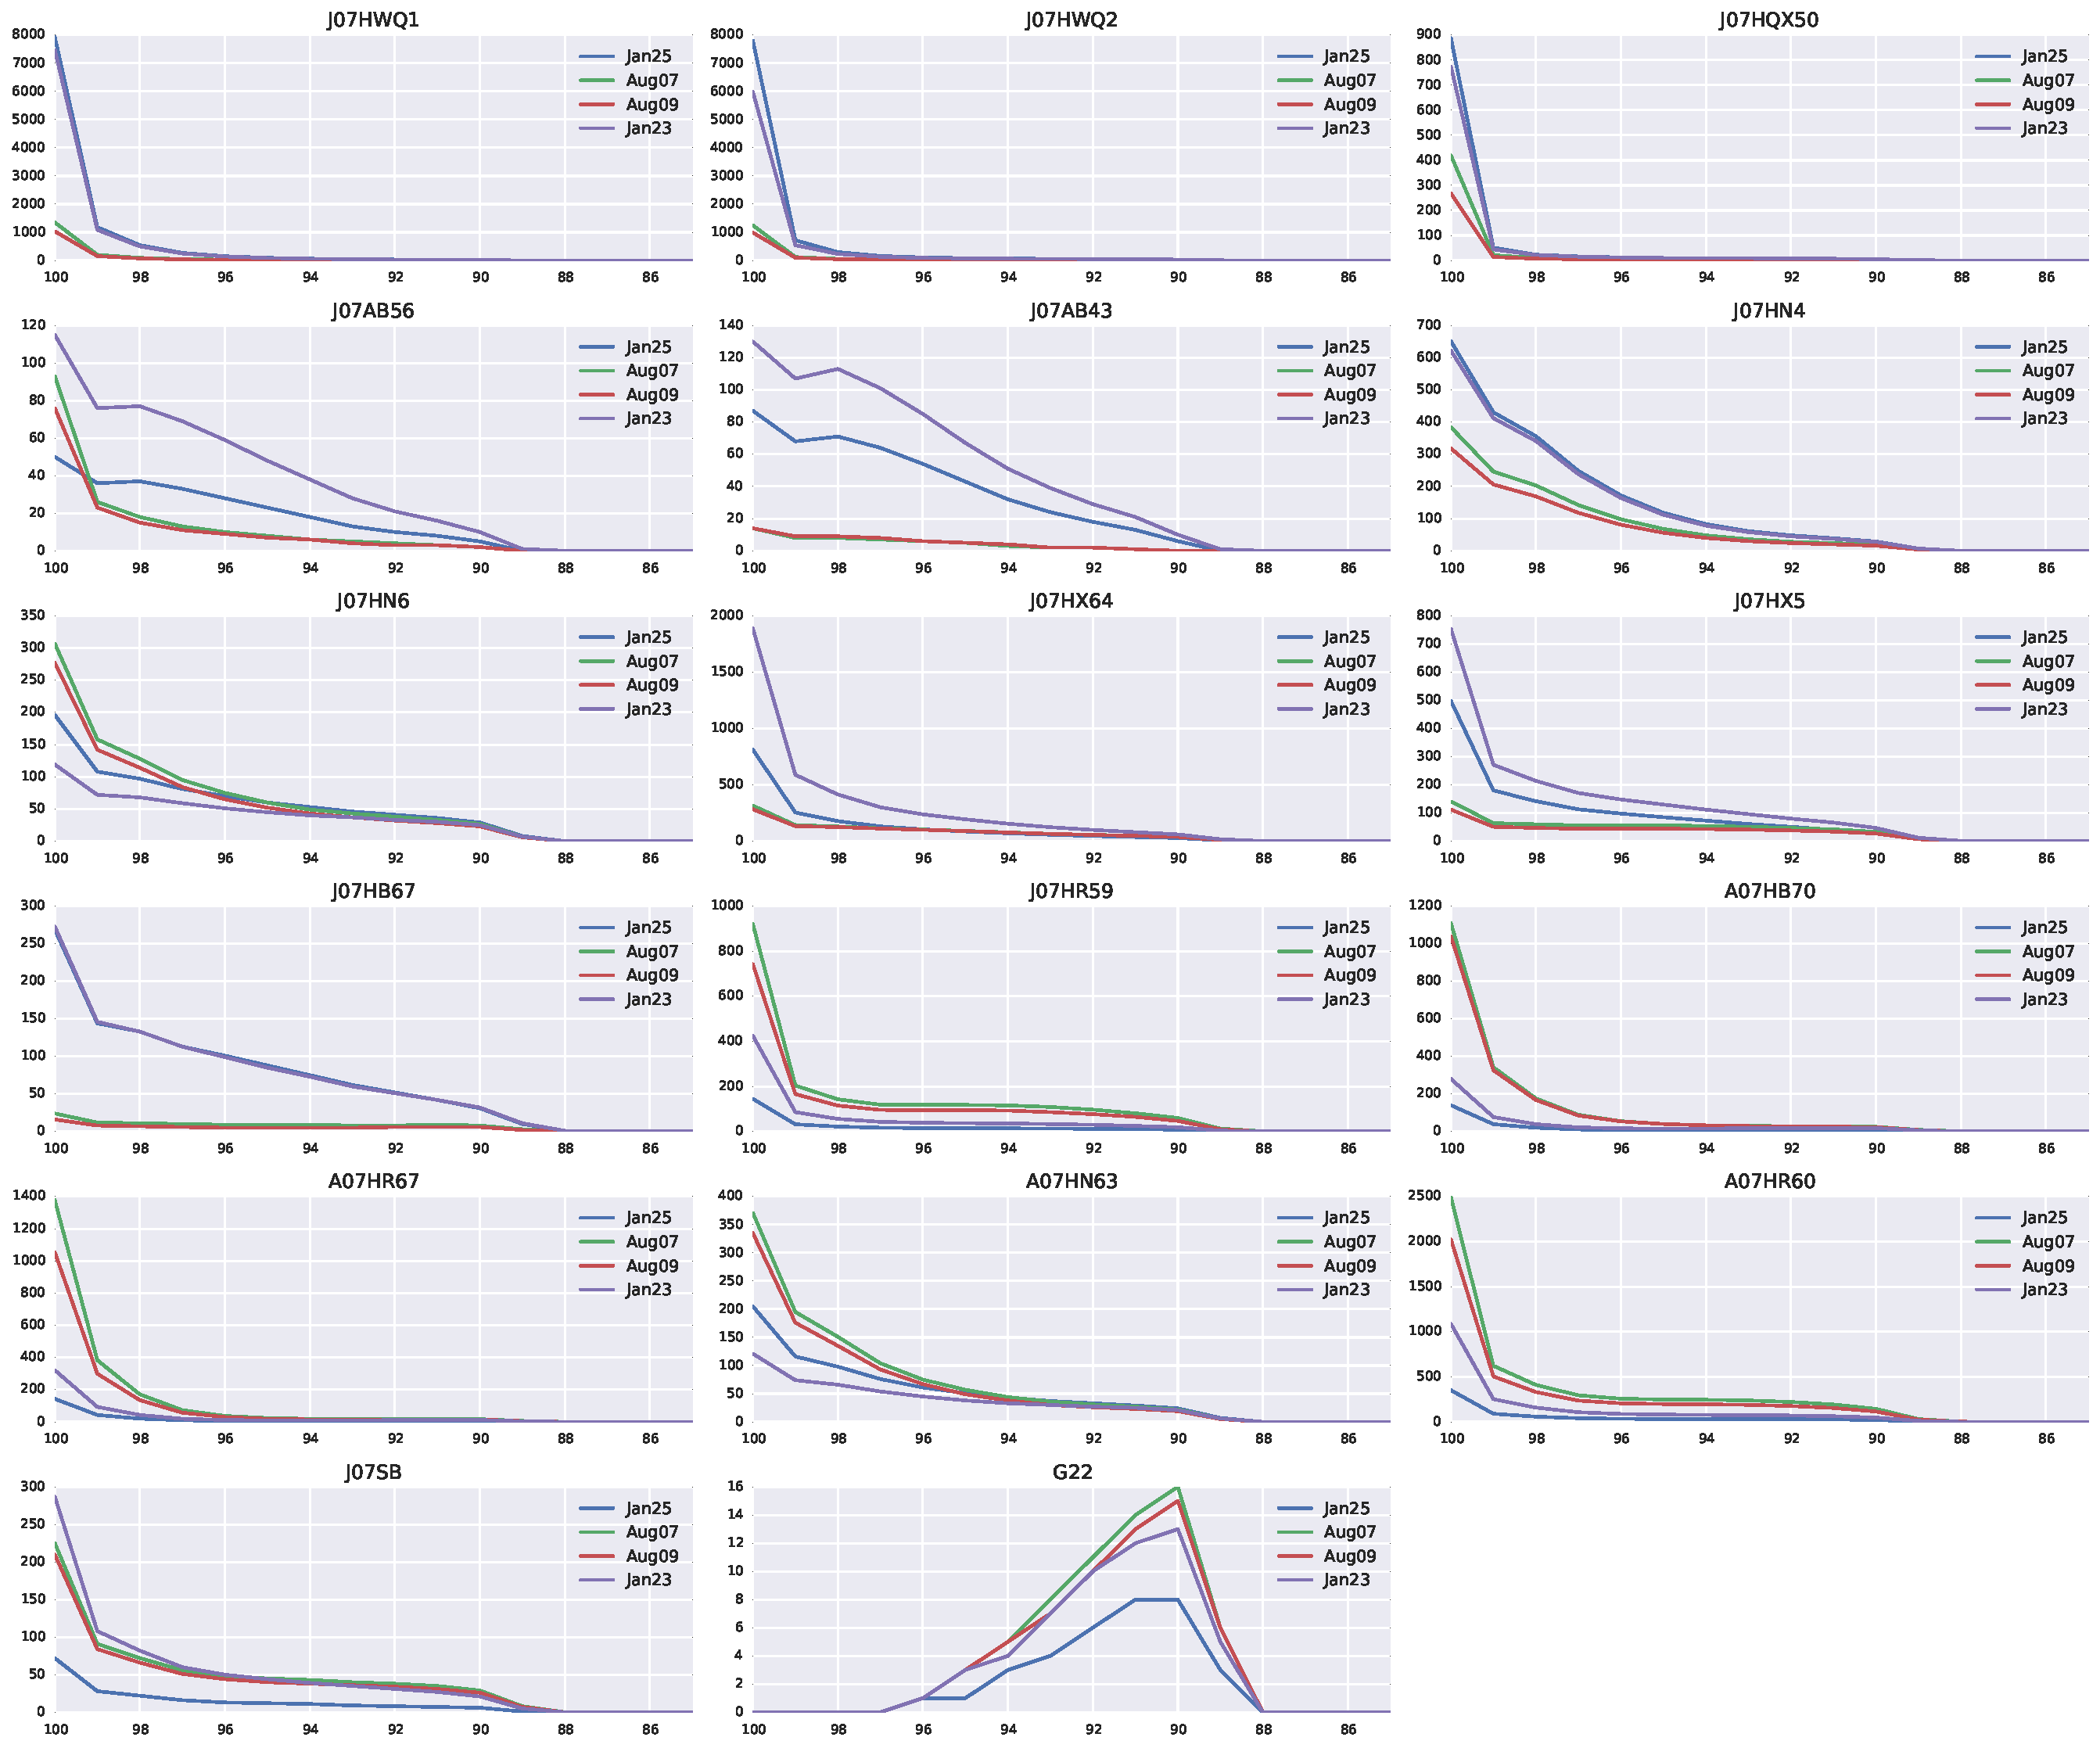
\includegraphics[width=\textwidth,height=\textwidth,keepaspectratio]{/Users/juan/Dropbox/GeneticVariationLT/Figures/GenomeIdentityPlots.pdf}
  \caption{Total number of recruited reads, grouped by identity. The X axis shows the identity of the read to the reference genome (\%), while the Y axis shows the number of reads recruited at that identity (thousands of reads).}
  \label{GenomeReadIdentity}
\end{figure}


%Figure Phylosift results
\begin{figure}[!hbtp]
\centering
\subfloat[Mapped reads]{
    \label{Jan23Mapped}
    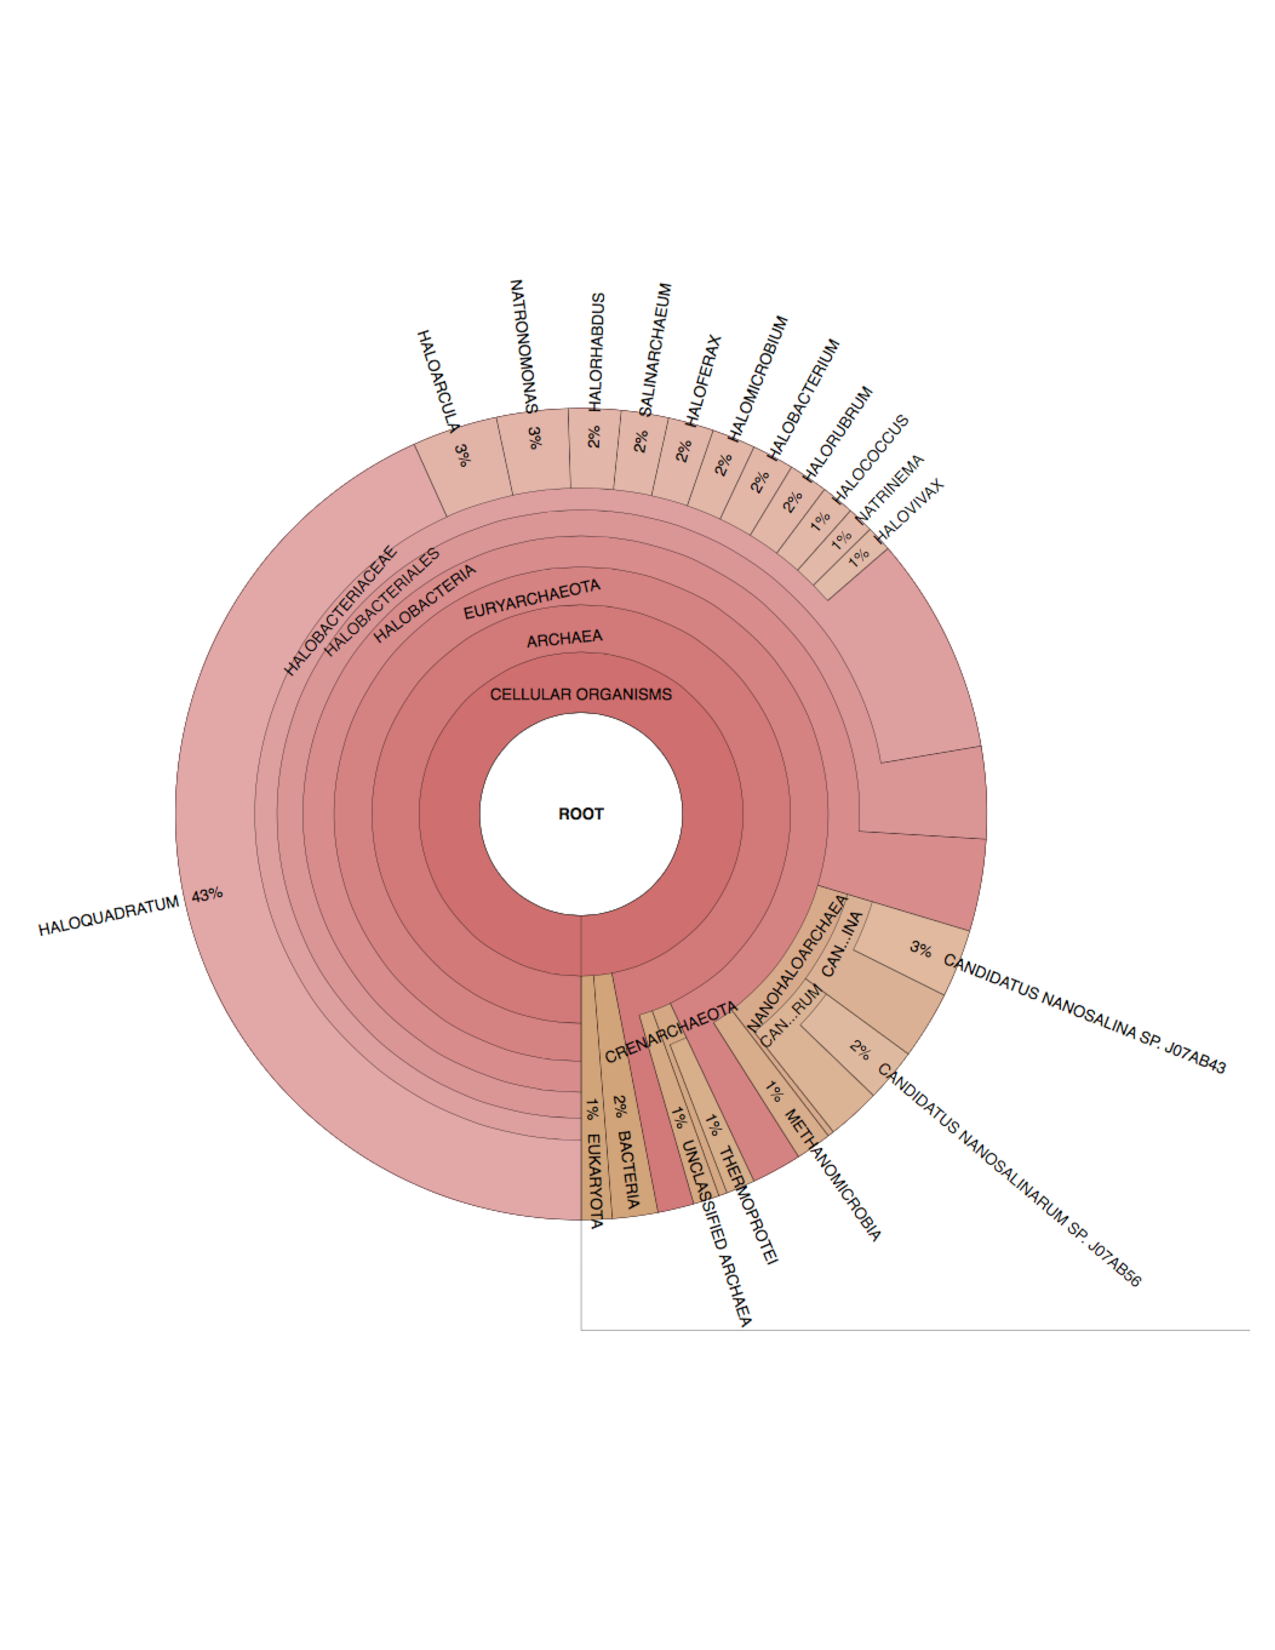
\includegraphics[width=0.7\textwidth]{Chapter5/Figures/Jan23_Mapped.pdf}
    }
    \hfill
\subfloat[Unmapped reads]{
    \label{Jan23Unmapped}
    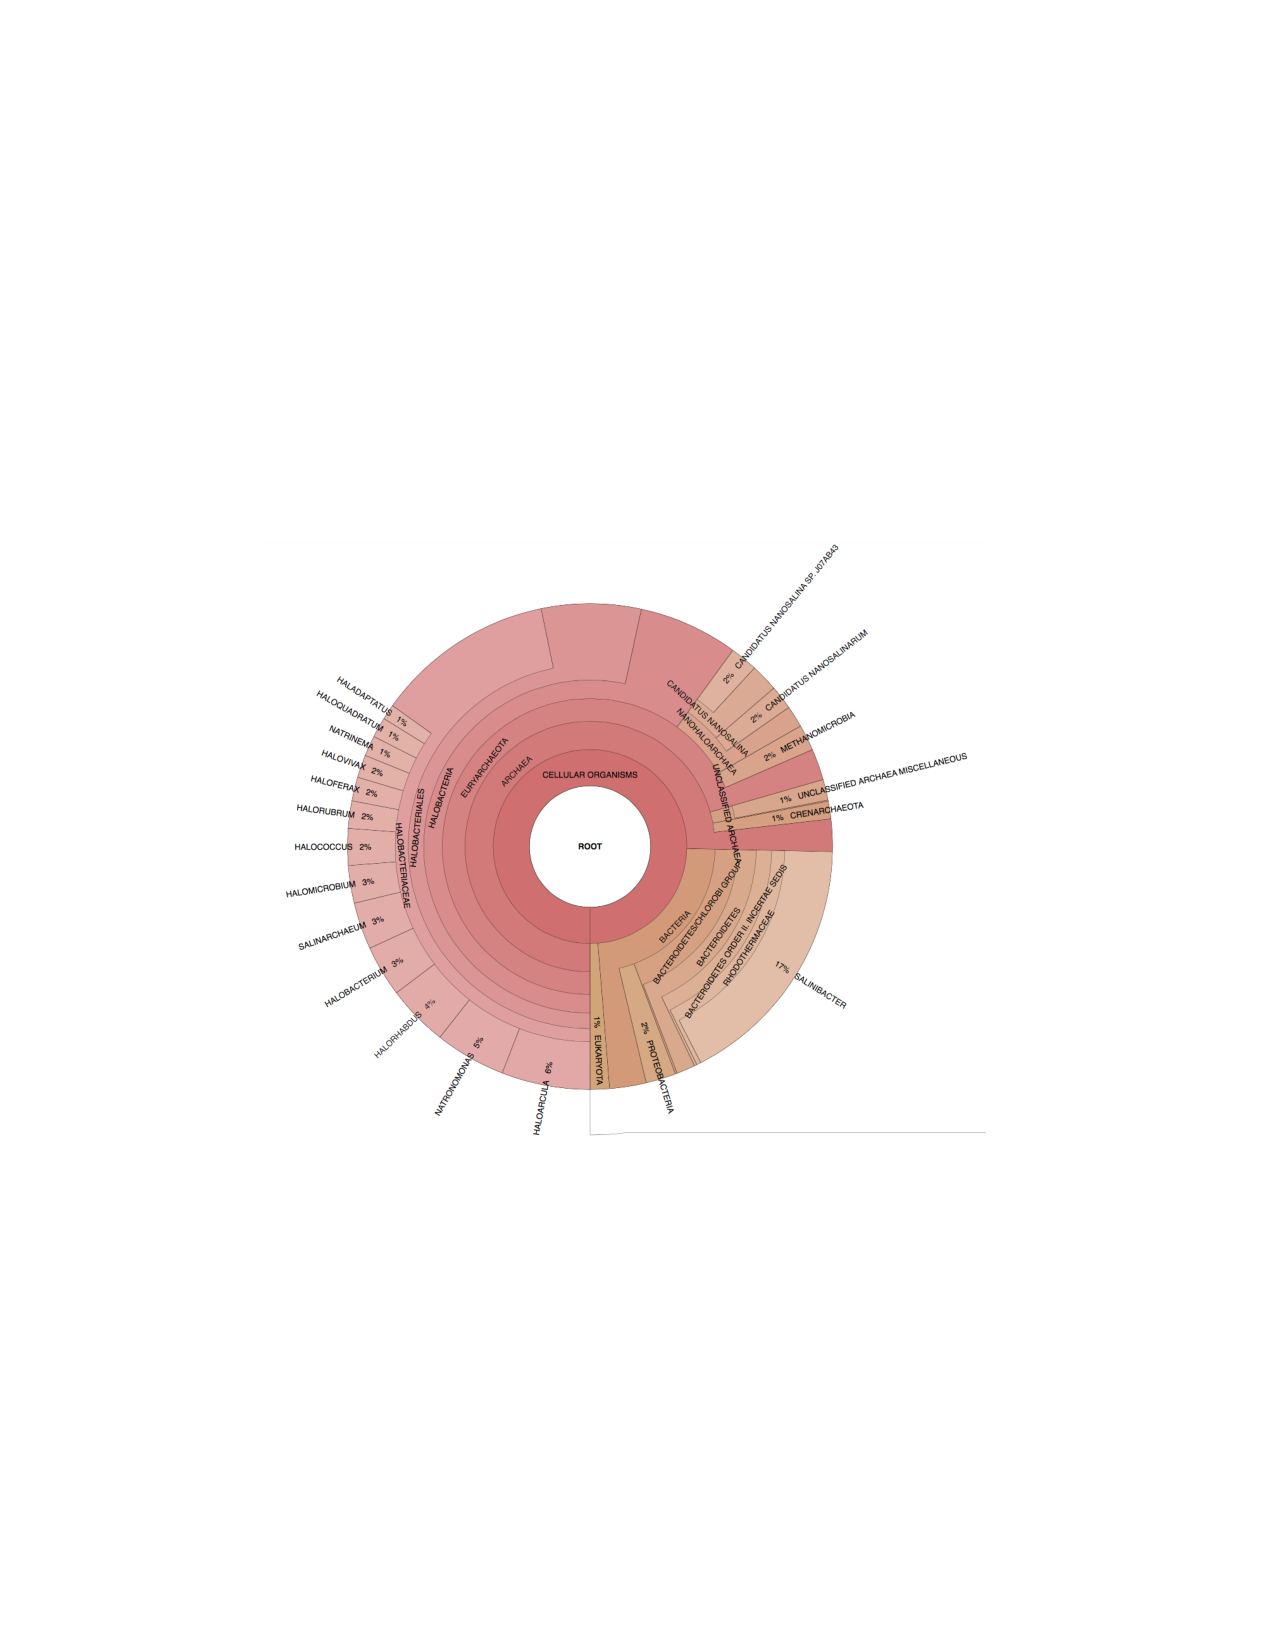
\includegraphics[width=0.7\textwidth]{Chapter5/Figures/Jan23_Unmapped.pdf}
    }
    \caption{Taxonomic classification of the mapped and unmapped reads using Phylosift \cite{Darling:2014ej}}
    \label{Jan23_Tax}
\end{figure}

%Figure Phylosift EPCA
\begin{figure}[hbt]
  \centering
  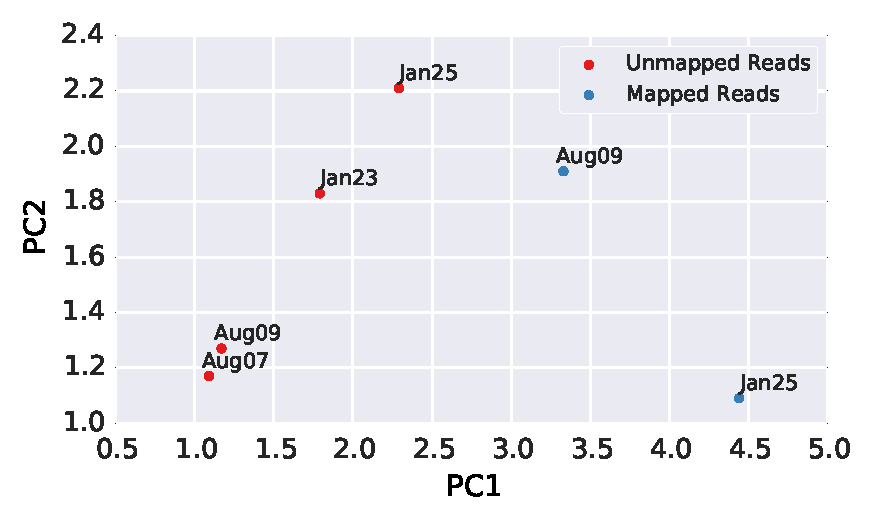
\includegraphics[width=\textwidth]{Chapter5/Figures/Unmapped_Mapped_EPCA.pdf}
  \caption{EPCA phylosift results}
  \label{EPCA_results}
\end{figure}


%%%%%%%%%%%%%%%%%%%%%%
\clearpage
\subsection{Genome coverage}



%Figure Gene differences season
\begin{figure}[!hbtp]
  \centering
  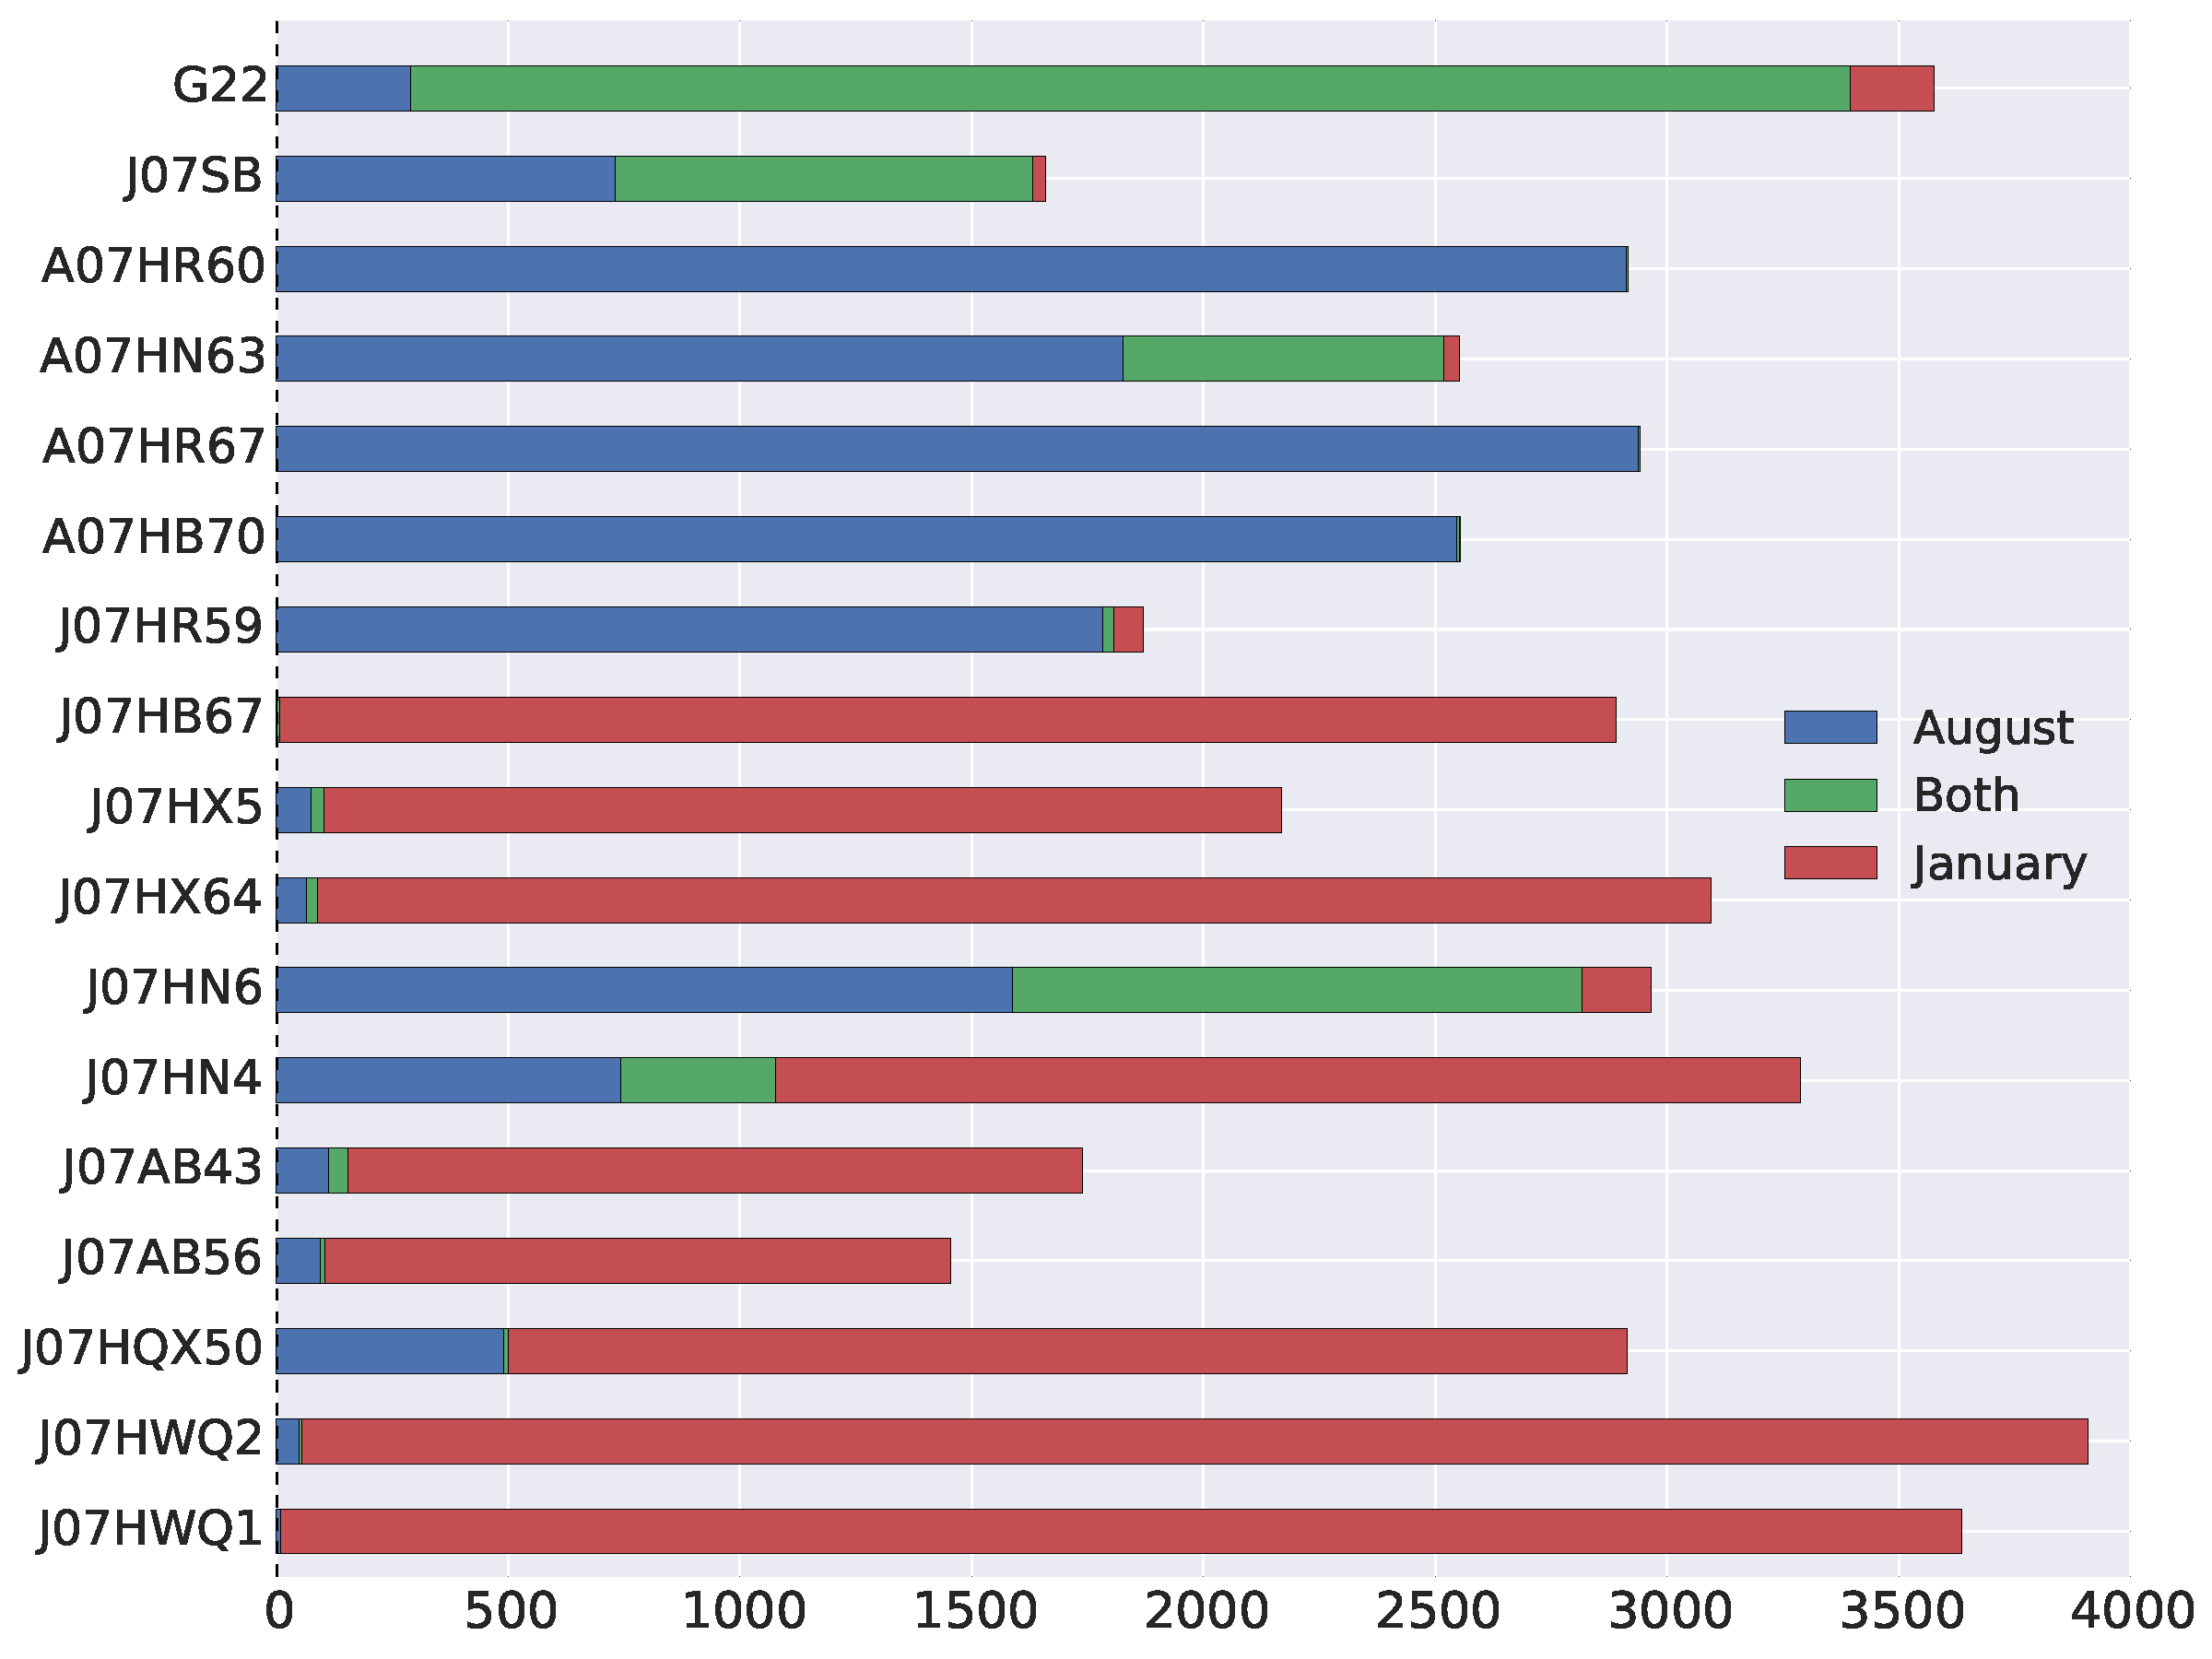
\includegraphics[width=0.9\textwidth]{Chapter5/Figures/GeneDifferencesSeason.pdf}
  \caption{Gene significant by seasons}
  \label{G22coverage}
\end{figure}



\subsection{Variation and positive selection analysis}

Results of the snps (\ref{SNPsummary}). Low number of SNPs for G22, so I'll leave out of the analysis. Reasons?
Comments about the trends?

Compariosn of the rate of SNPs (independent of the type). DONE (Table)

Venn diagram of the SNPs, can we collapse January samples and August samples. DONE


Genes with most of the SNPs
Genes with no SNPs 
Use BEDTOOLS ANNOTATE FOR THIS



Dn/DS
network diagram of DN/ds and selection, january versus august


\begin{table}[hbt]
  \caption{Change rate for SNPs}
  \begin{tabularx}{\textwidth}{L{2.2cm}R{2cm}R{3cm}R{3.2cm}R{2cm}}
  \hline
    \textbf{Genome} & \textbf{Jan 23} & \textbf{Jan 25} & \textbf{Aug 07} & \textbf{Aug 09} \\
    \hline
     \textit{J07HWQ1} & 261 & 262 & 267 & 270 \\
     \textit{J07HWQ2} & 398 & 397 & 305 & 407 \\
     \textit{J07HQX50} & 695 & 693 & 706 & 718 \\
     \textit{J07AB56} & 99 & 103 & 202 & 192 \\
     \textit{J07AB43} & 93 & 94 & 137 & 139 \\
     \textit{J07HN4} & 110 & 110 & 111 & 111 \\
     \textit{J07HN6} & 348 & 383 & 351 & 356 \\
     \textit{J07HX64} & 105 & 106 & 107 & 108 \\
     \textit{J07HX5} & 108 & 109 & 110 & 111 \\
     \textit{J07HB67} & 110 & 109 & 155 & 191 \\
     \textit{J07HR59} & 738 & 872 & 651 & 663 \\
     \textit{A07HB70} & 139 & 142 & 137 & 137 \\
     \textit{A07HR67} & 171 & 175 & 169 & 169 \\
     \textit{A07HN63} & 581 & 504 & 471 & 476 \\
     \textit{A07HR60} & 264 & 271 & 256 & 257 \\
     \textit{G22} & 24,126 & 33,241 & 29,898 & 31,227 \\
     \textit{J07SB} & 165 & 177 & 164 & 164 \\     
  \end{tabularx}
  \label{ChangeRate}
\end{table}

%FIgures. SNP summary
\begin{figure}[!hbtp]
  \centering
  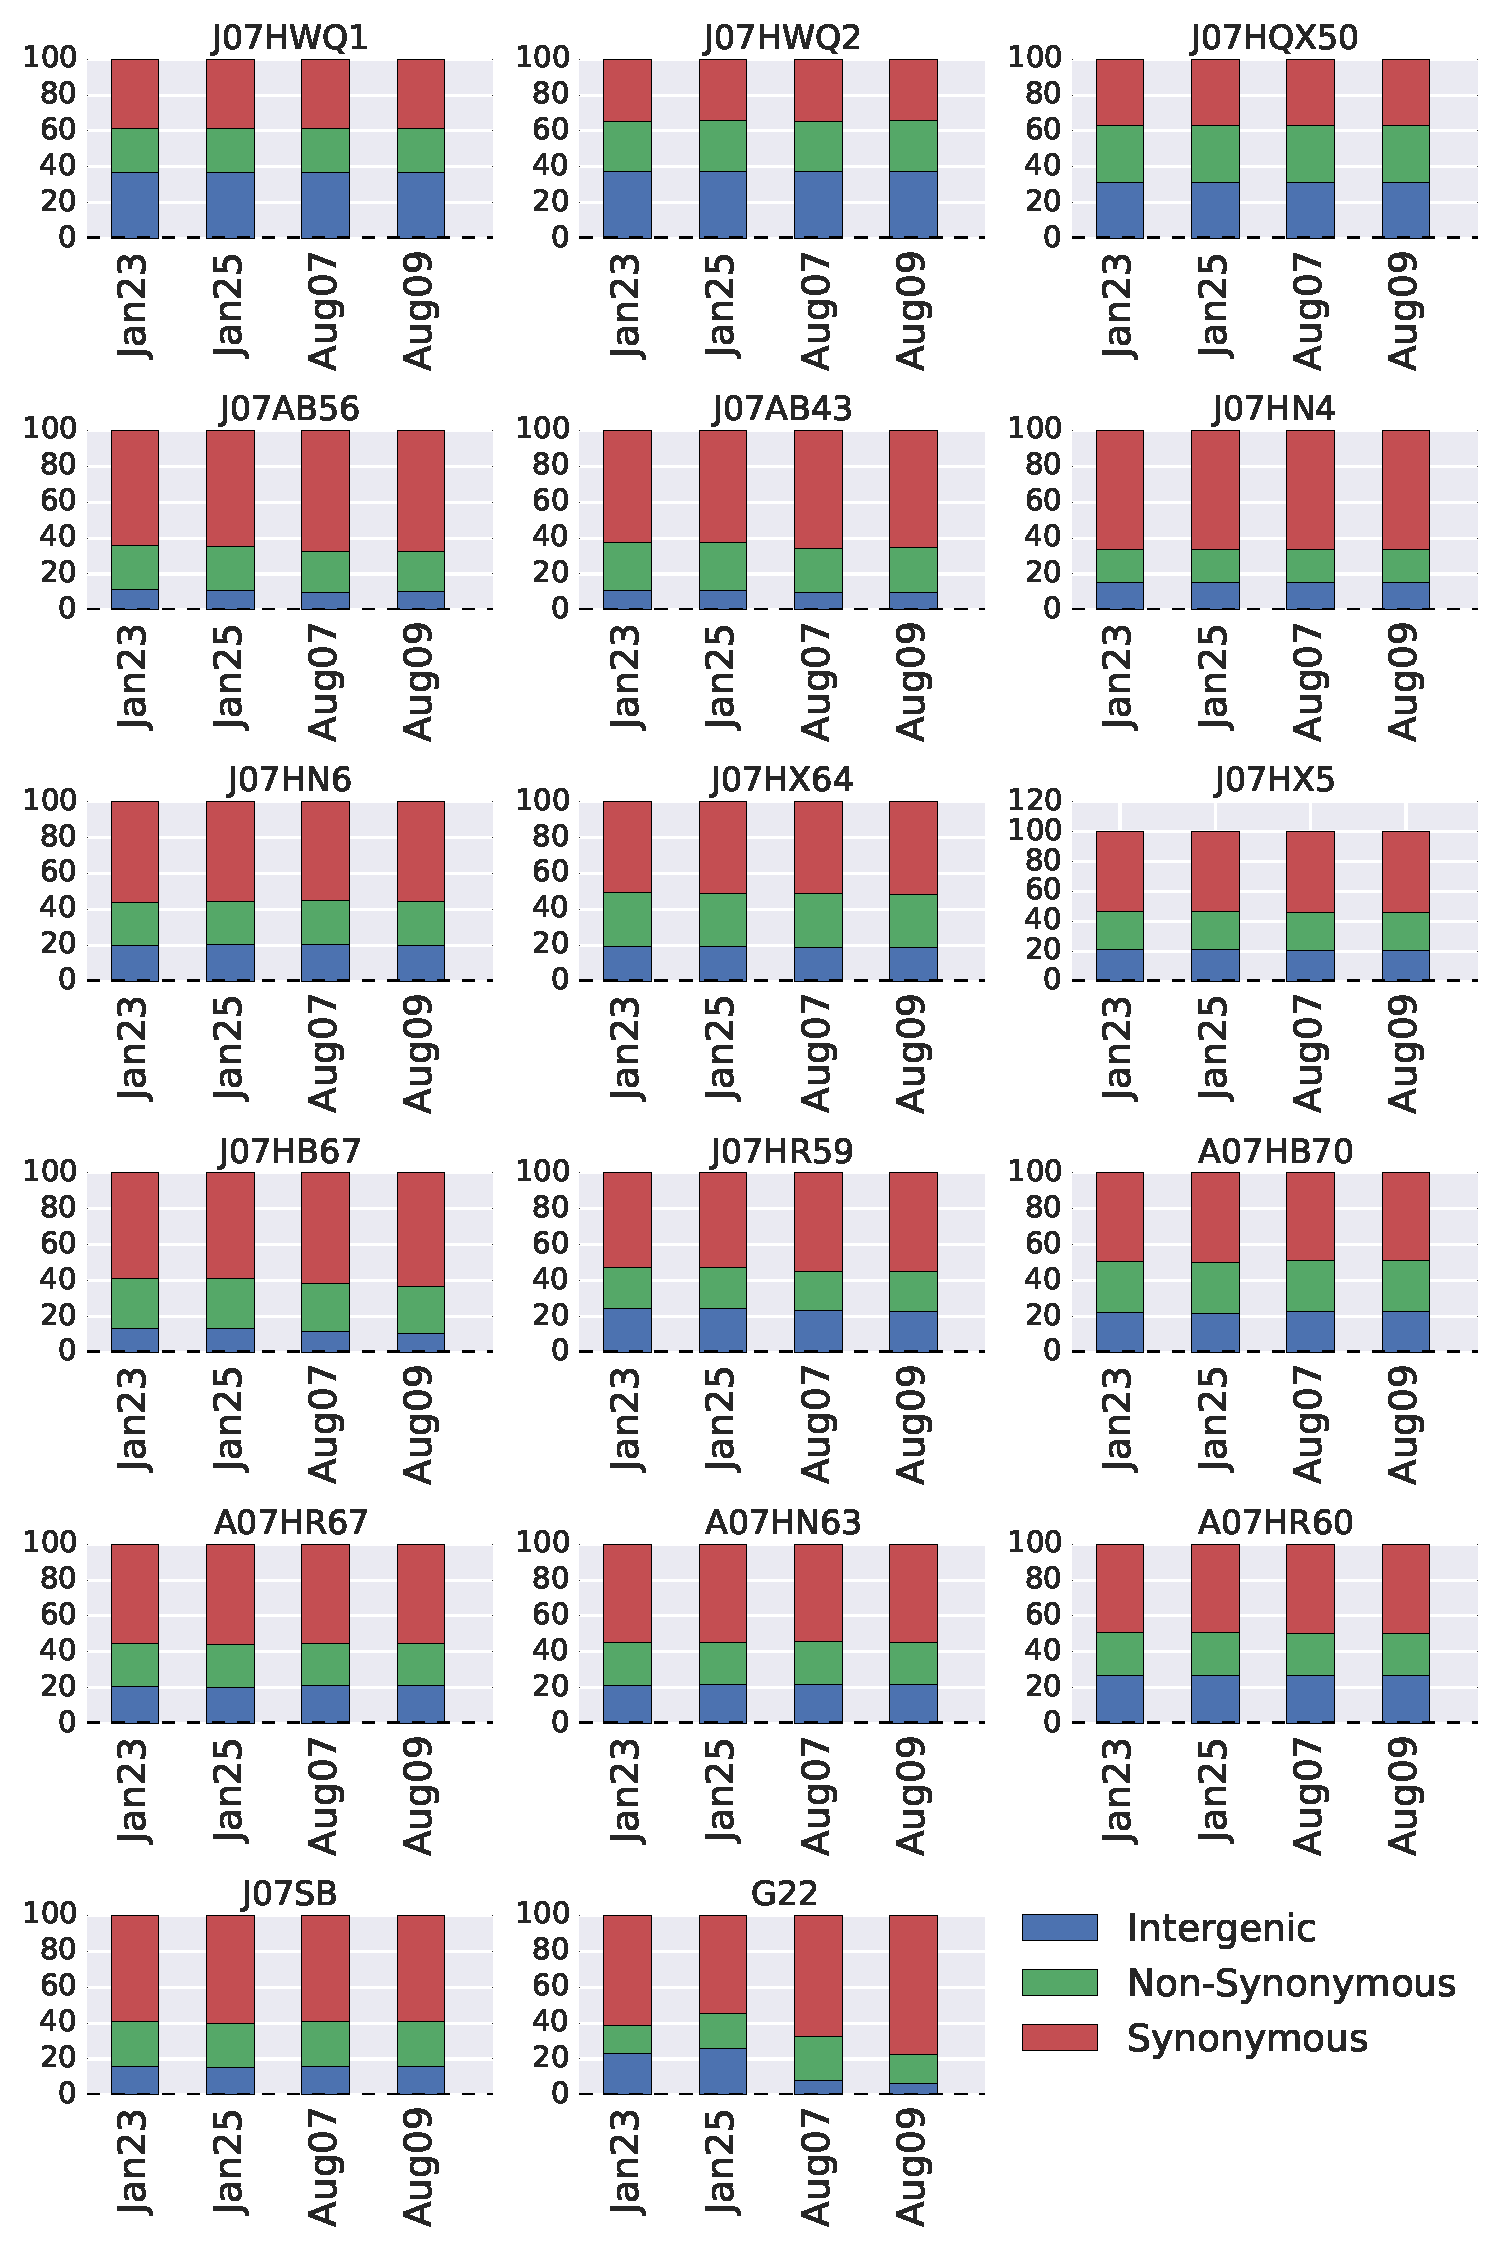
\includegraphics[width=\textwidth]{Chapter5/Figures/SNPsummary.pdf}
  \caption{SNPsummary}
  \label{SNPSummary}
\end{figure}

%Figure VENN diagram January
\begin{figure}[!hbtp]
  \centering
  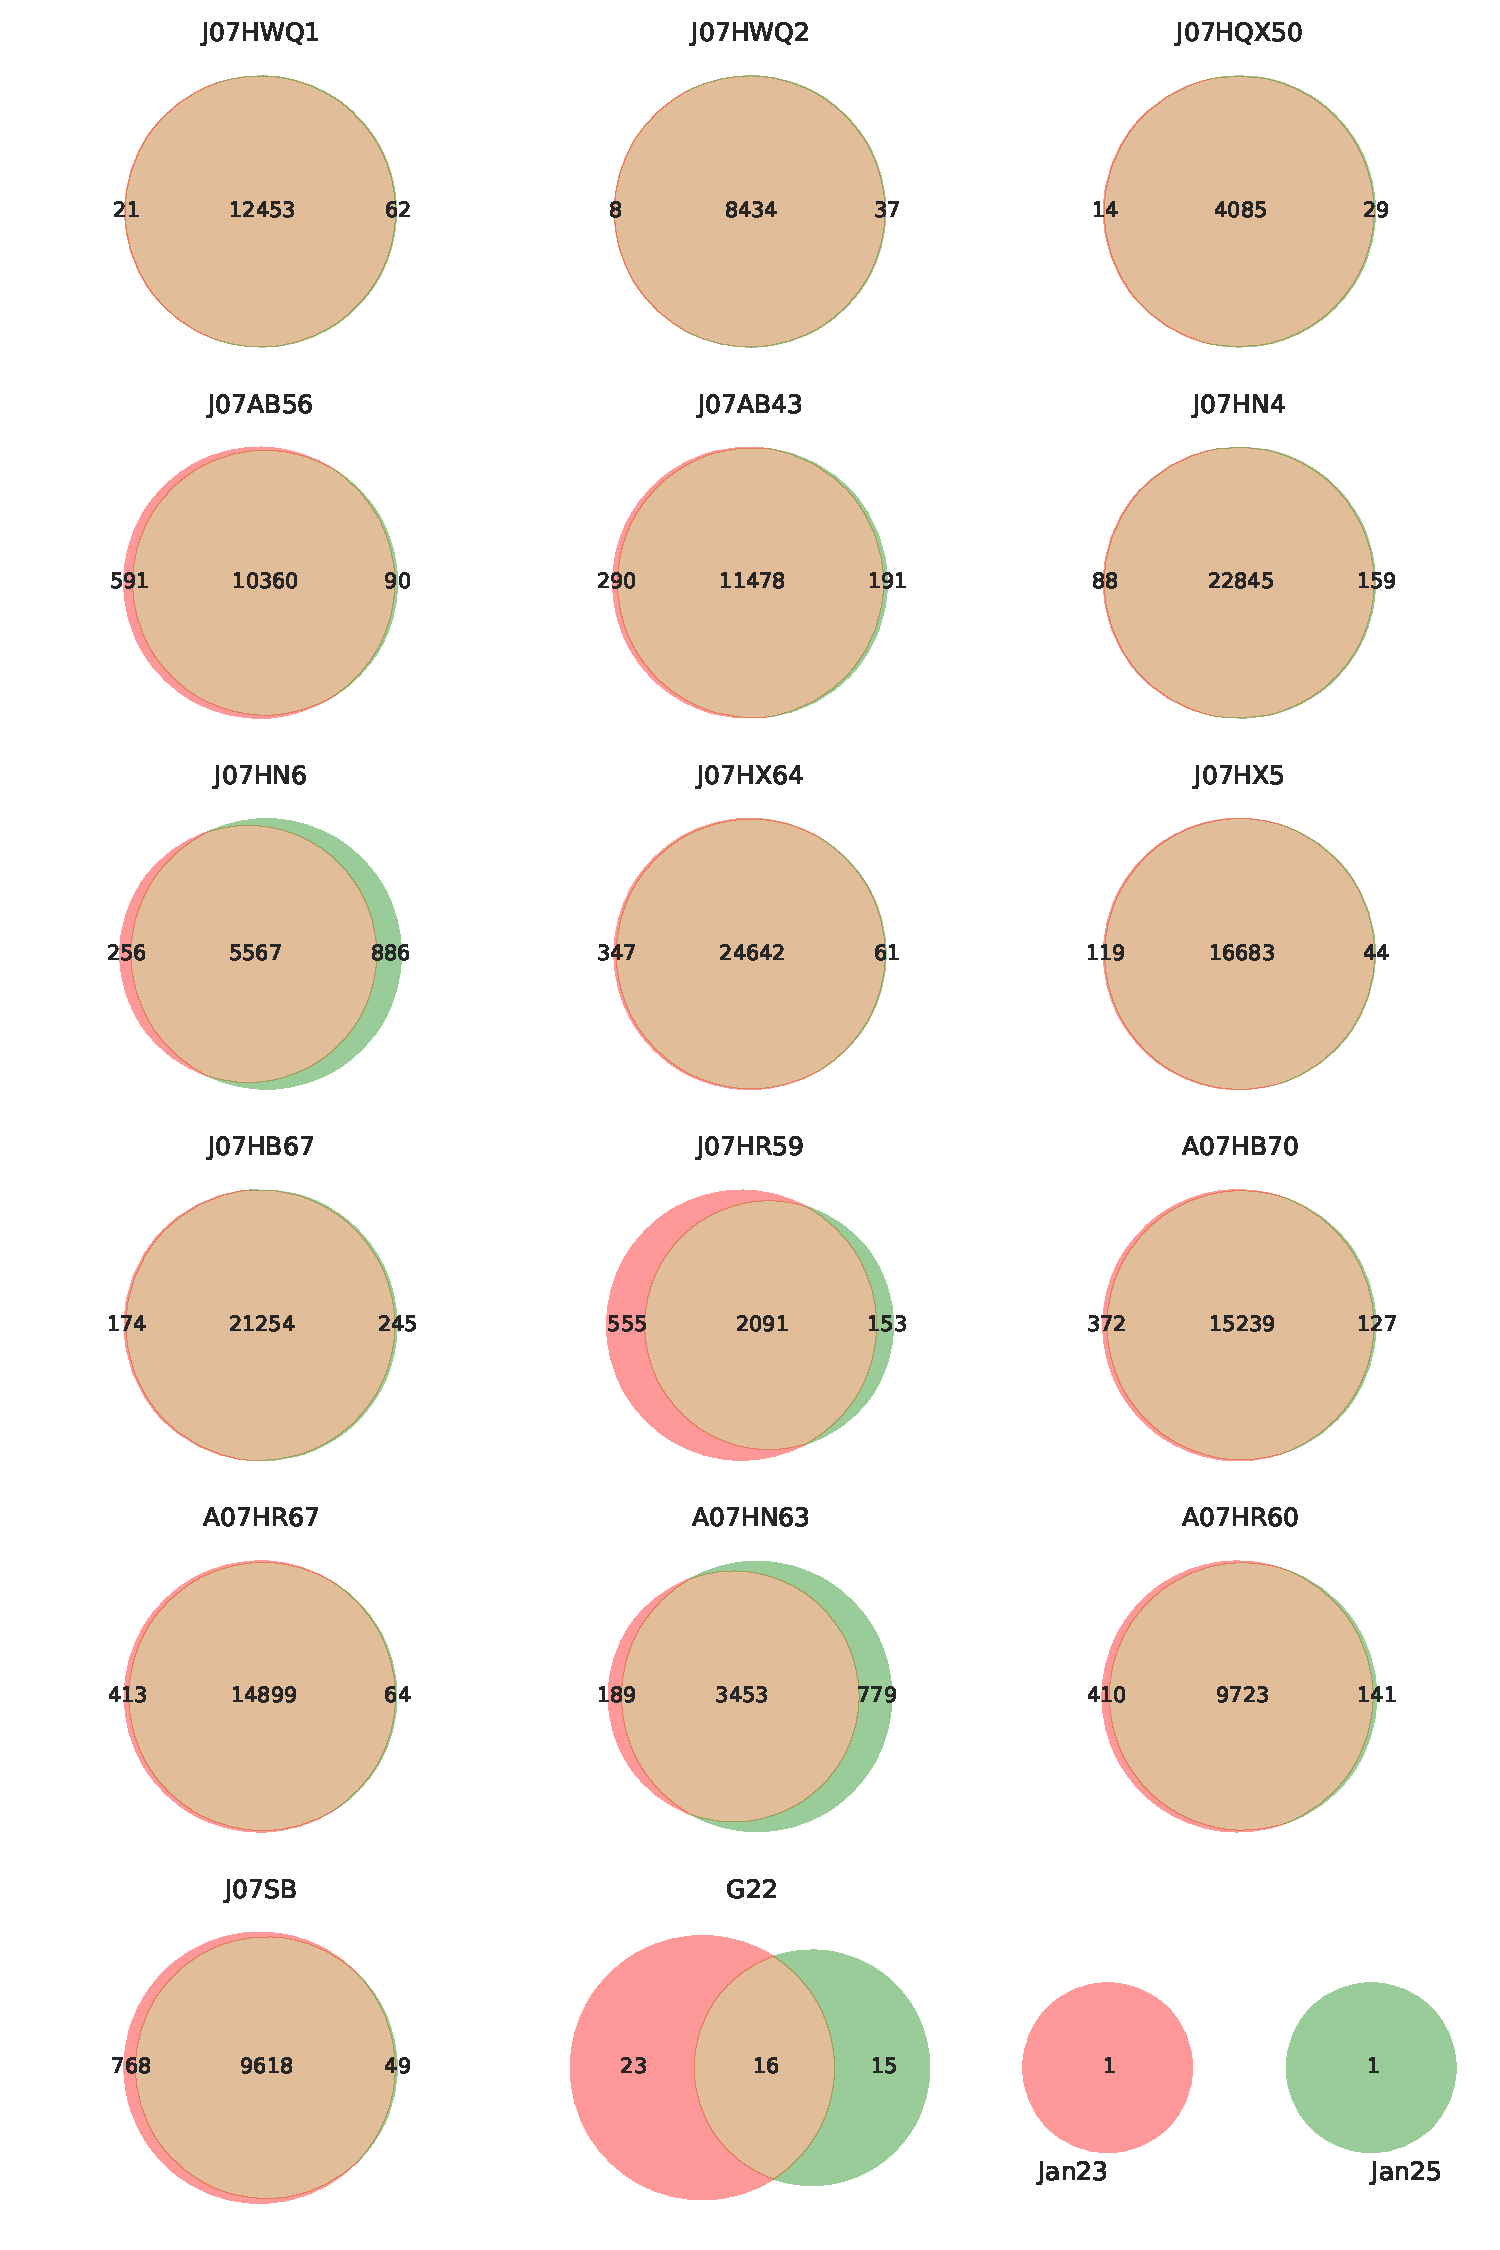
\includegraphics[width=\textwidth]{Chapter5/Figures/Venn_JanuarySNPs.pdf}
  \caption{JanuarySNPs}
  \label{VennJan}
\end{figure}

%VENN diagram August
\begin{figure}[!hbtp]
  \centering
  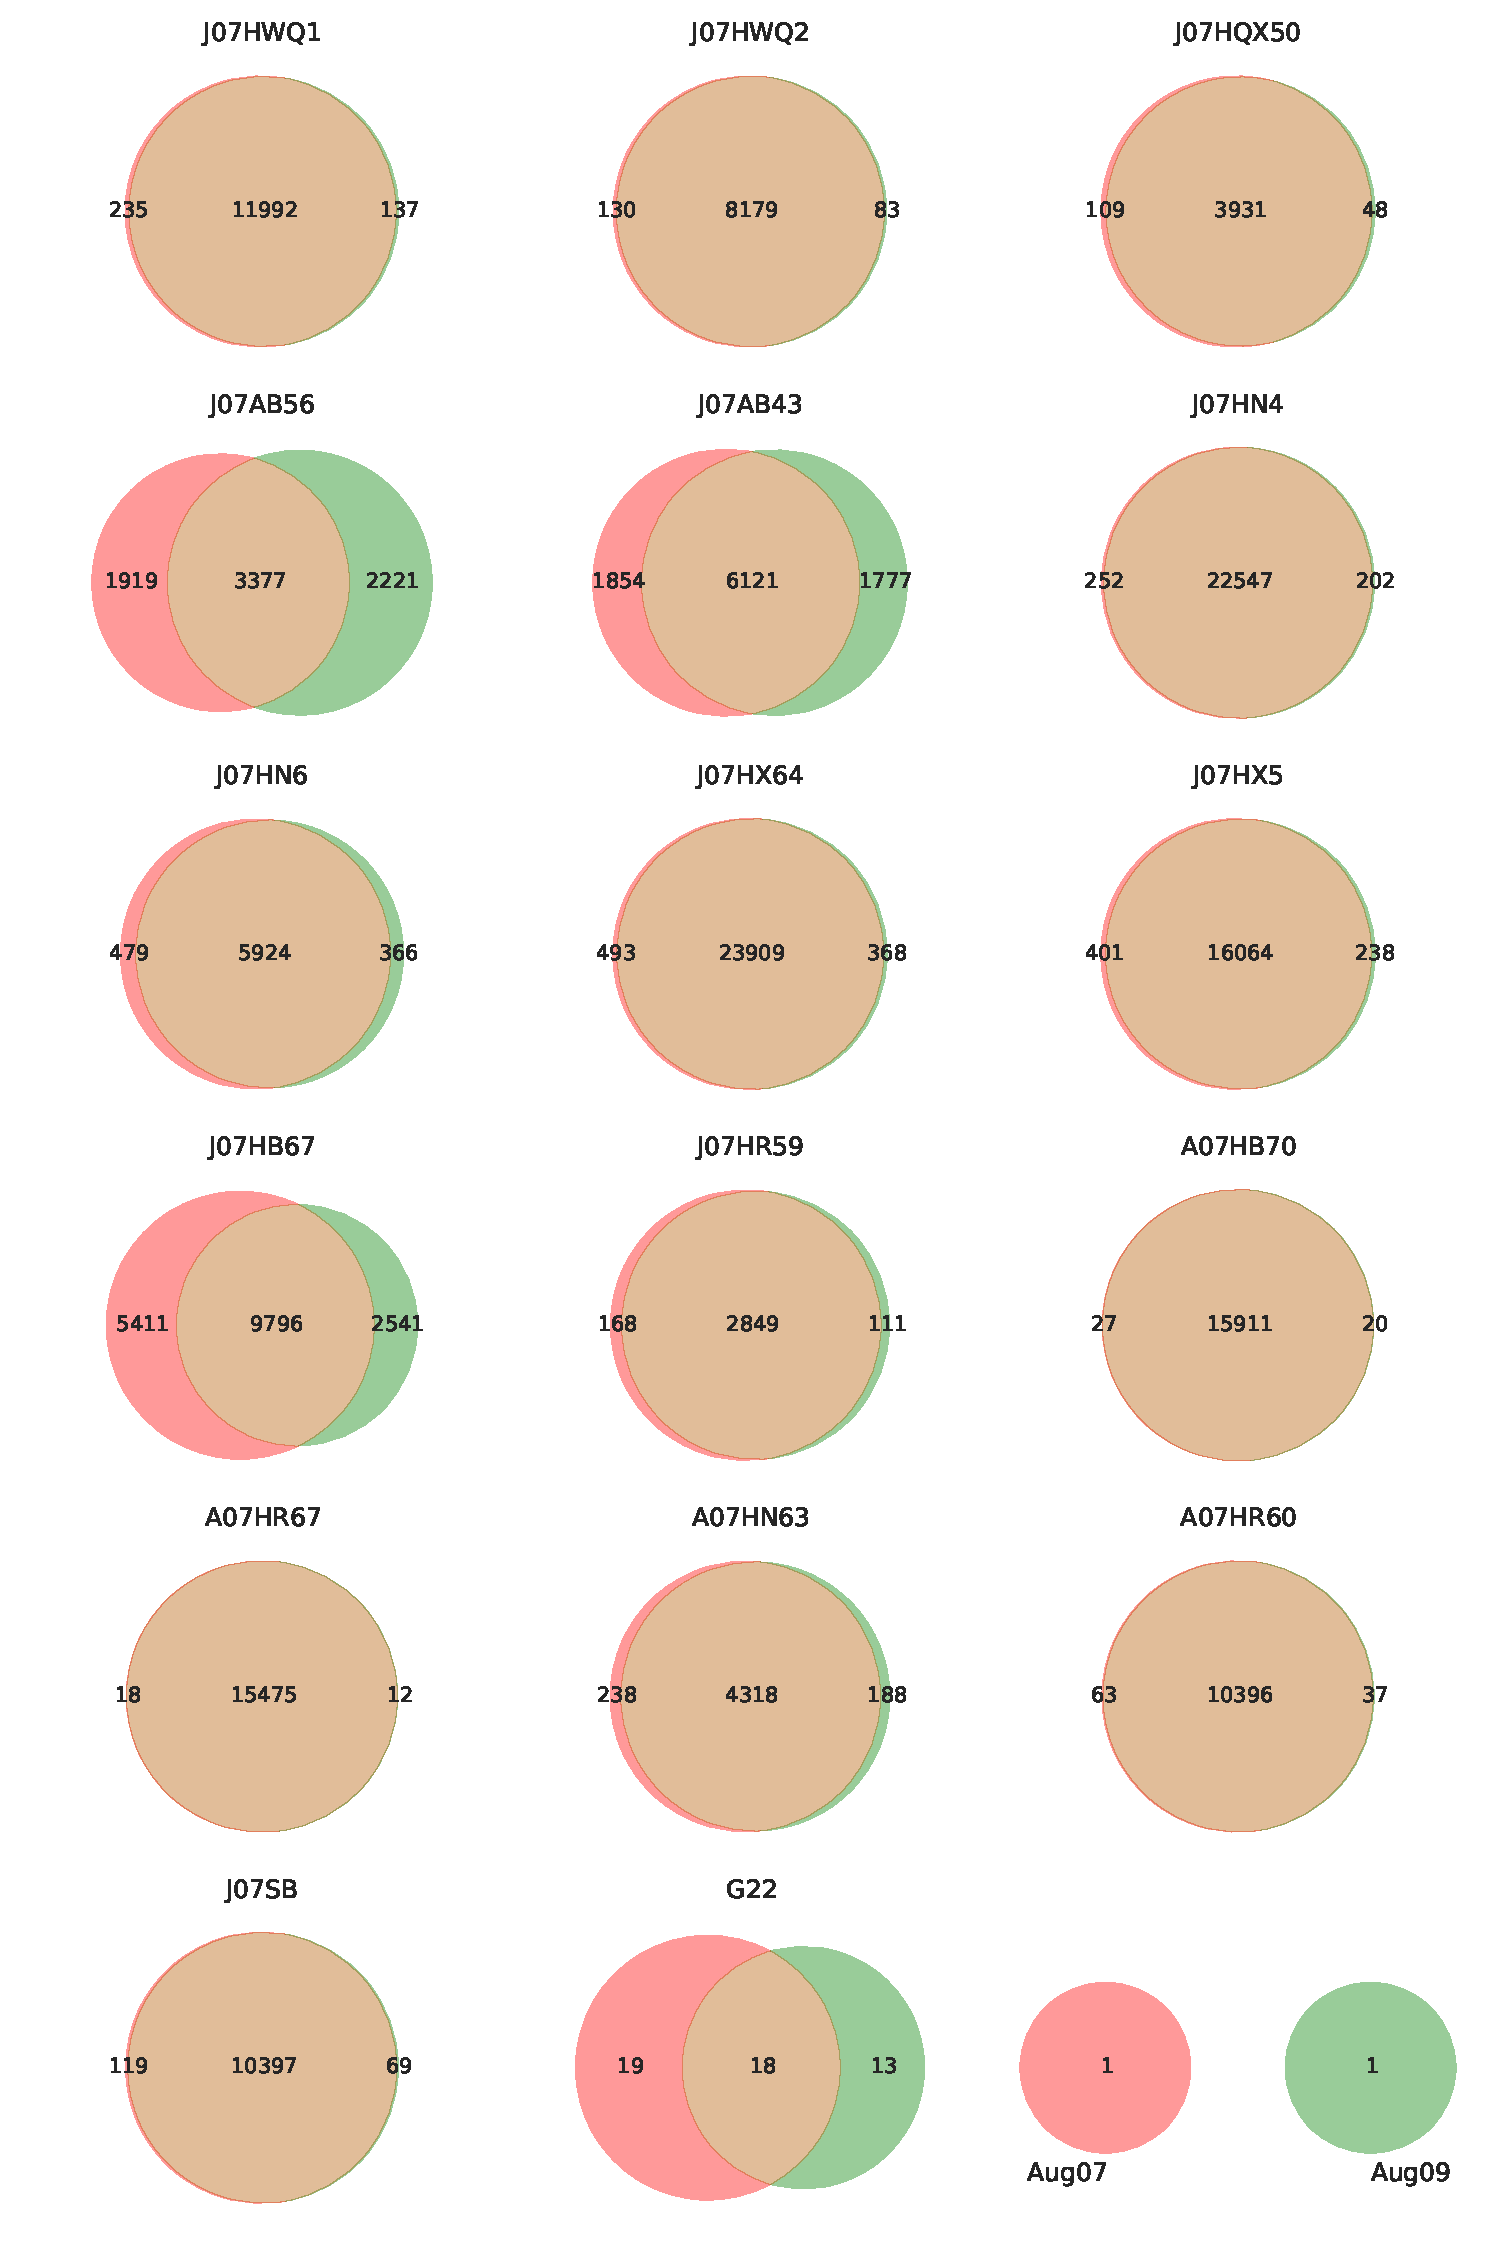
\includegraphics[width=\textwidth]{Chapter5/Figures/Venn_AugustSNPs.pdf}
  \caption{AugustSNPs}
  \label{VennAug}
\end{figure}

%VENN digram both
\begin{figure}[!hbtp]
  \centering
  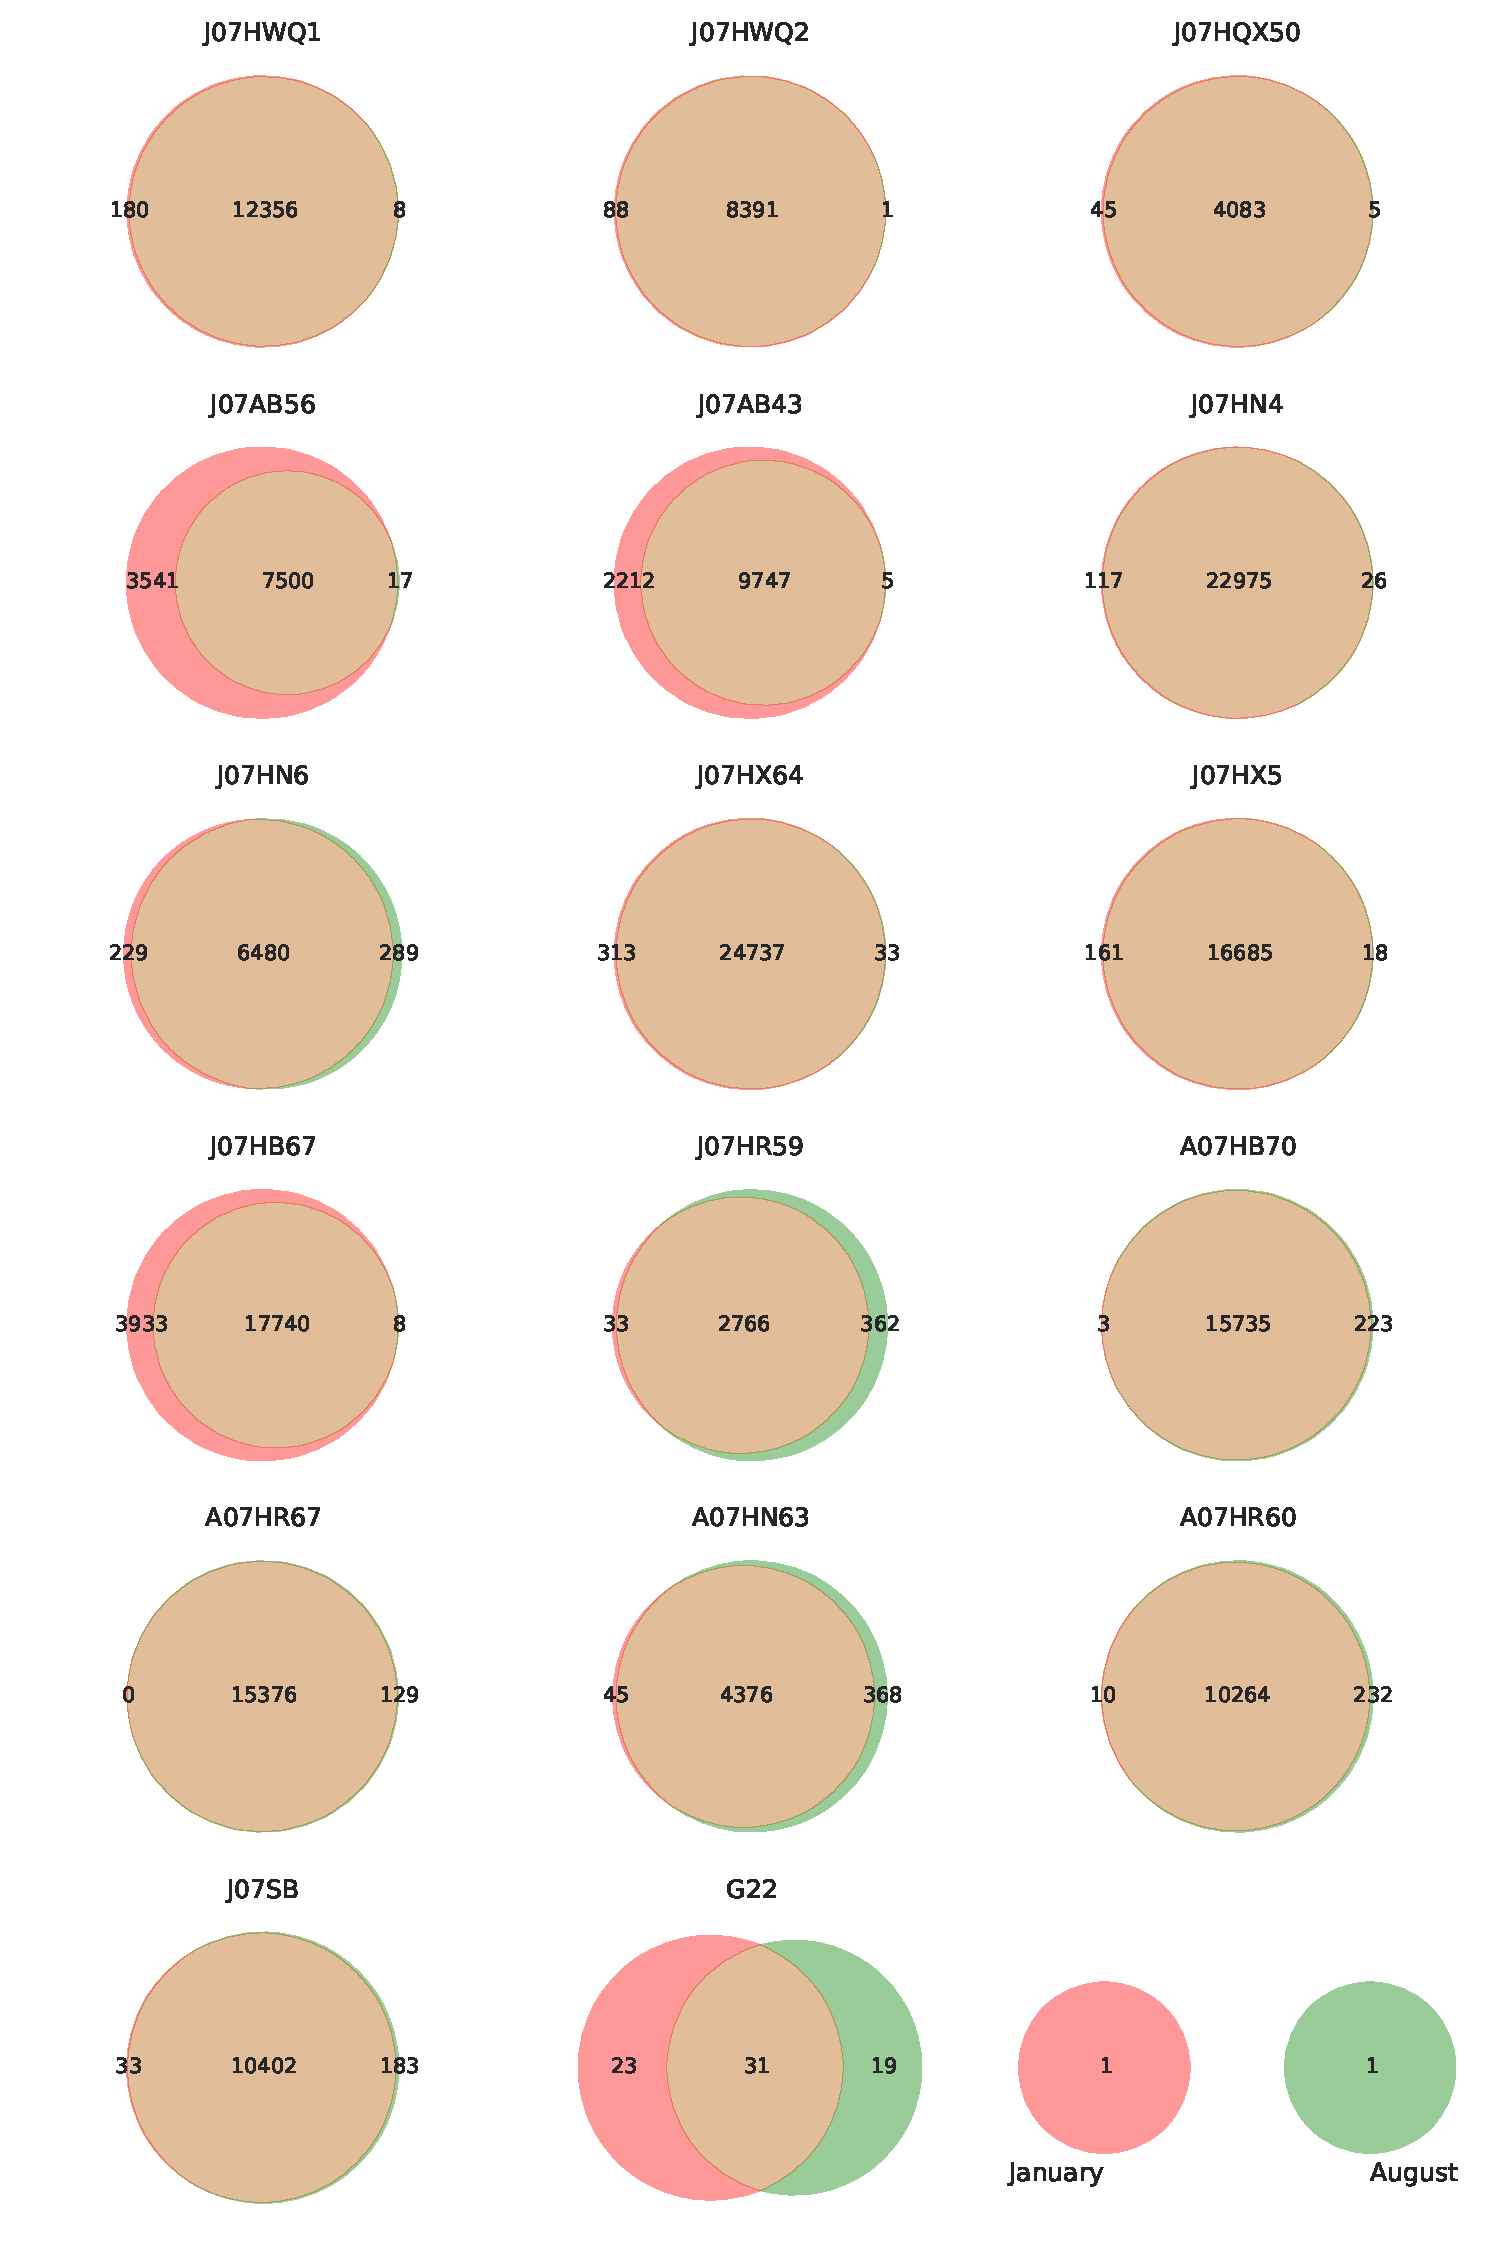
\includegraphics[width=\textwidth]{Chapter5/Figures/Venn_JanAugSNPs.pdf}
  \caption{BothSNPs}
  \label{VennBoth}
\end{figure}

%SNP frequency plot
\begin{figure}[!hbtp]
  \centering
  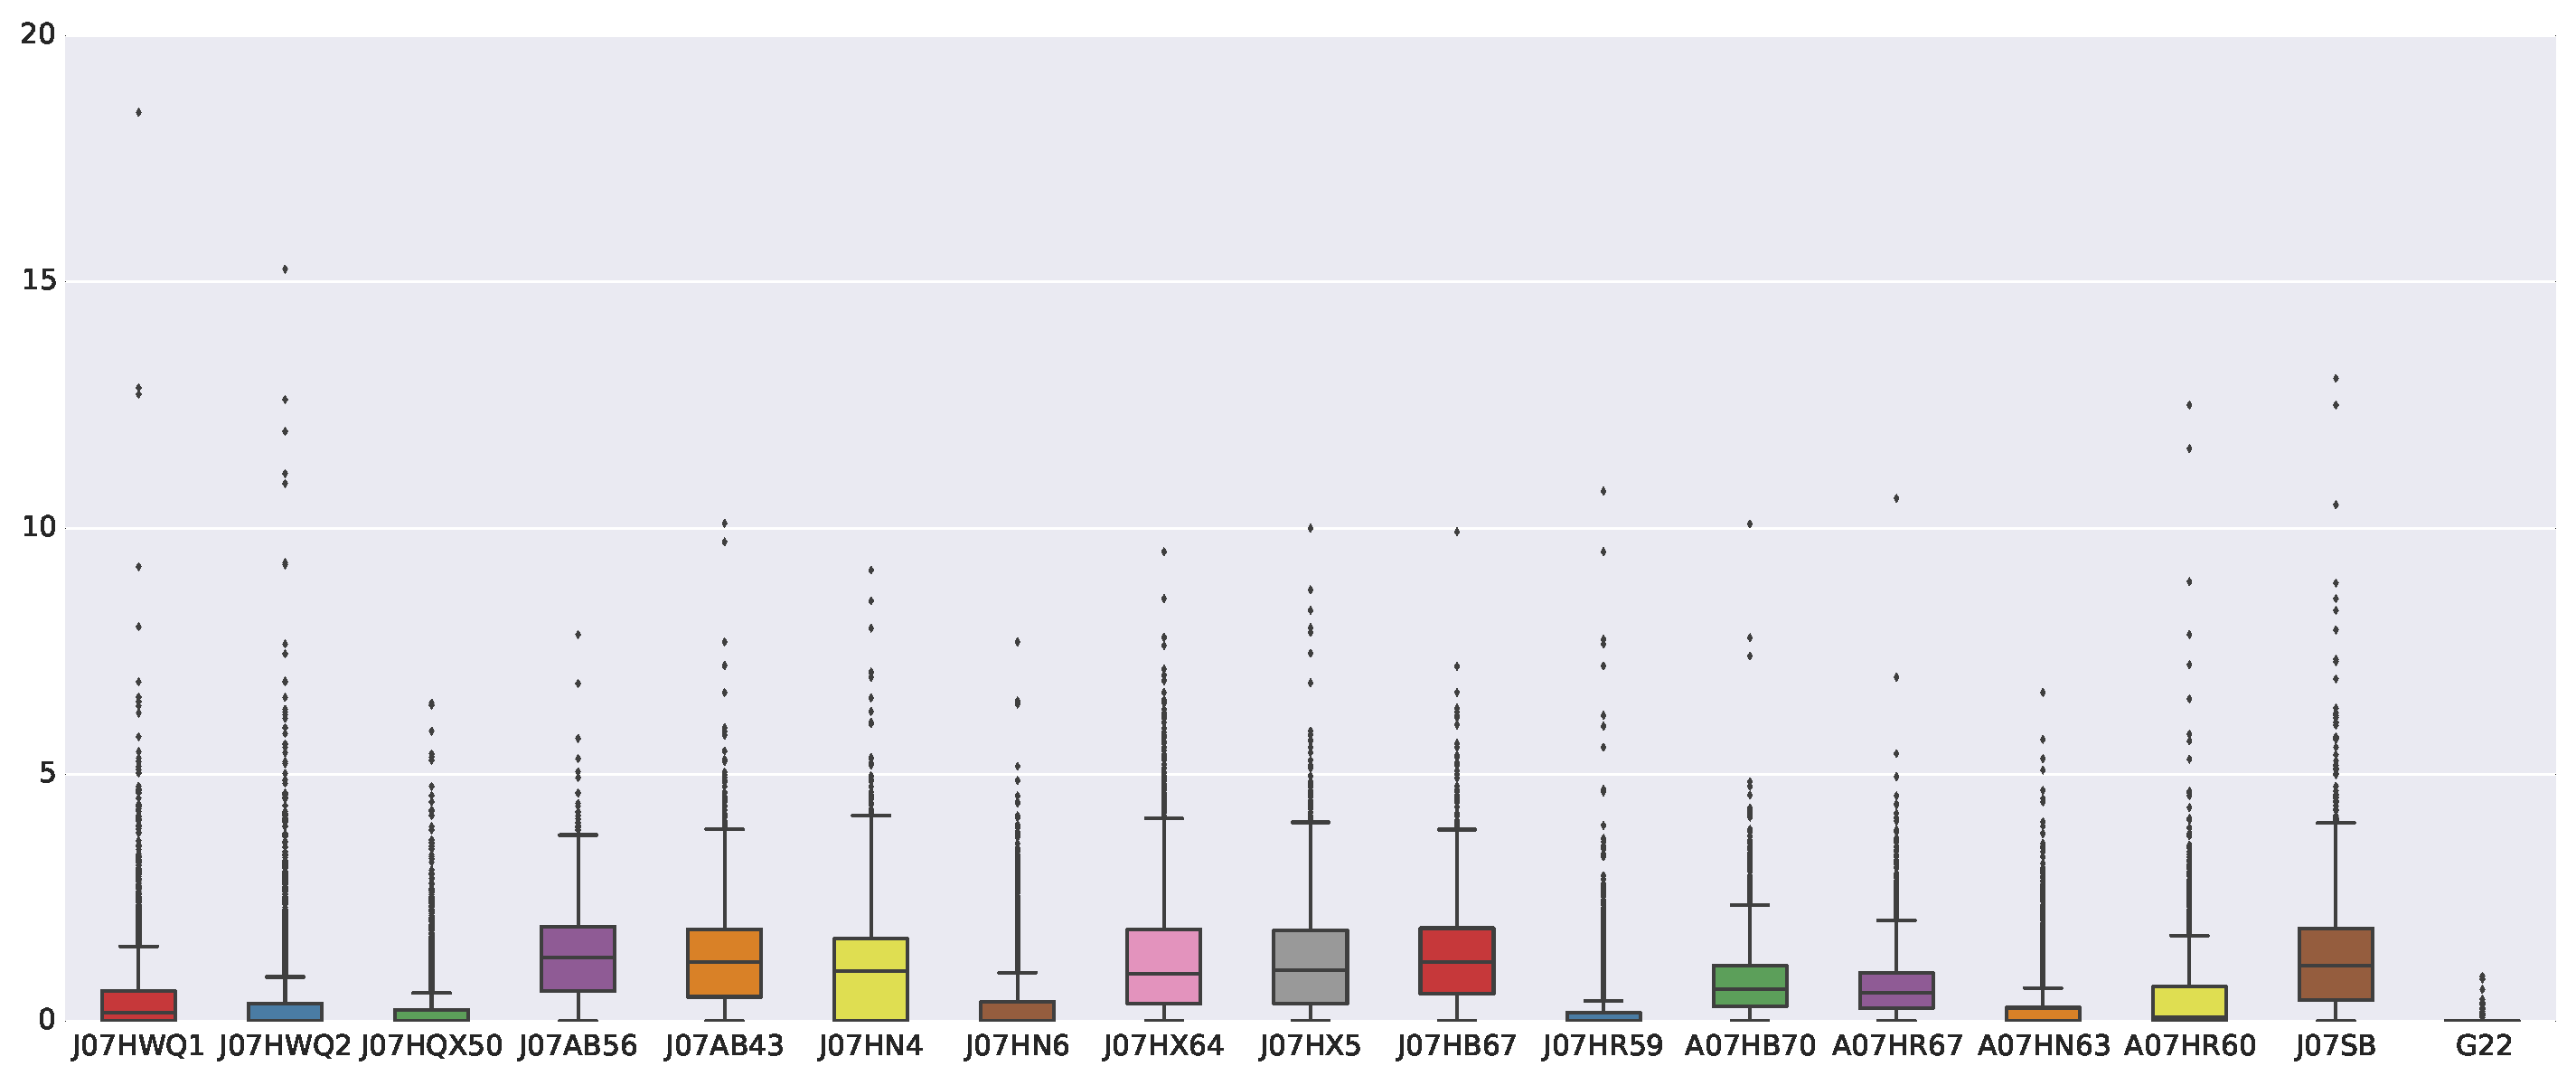
\includegraphics[width=\textwidth]{Chapter5/Figures/SNP_freq_boxplot.pdf}
  \caption{SNpp frequency}
  \label{SNP_boxplot}
\end{figure}

%Figure Mapping
\begin{figure}[!hbtp]
  \centering
  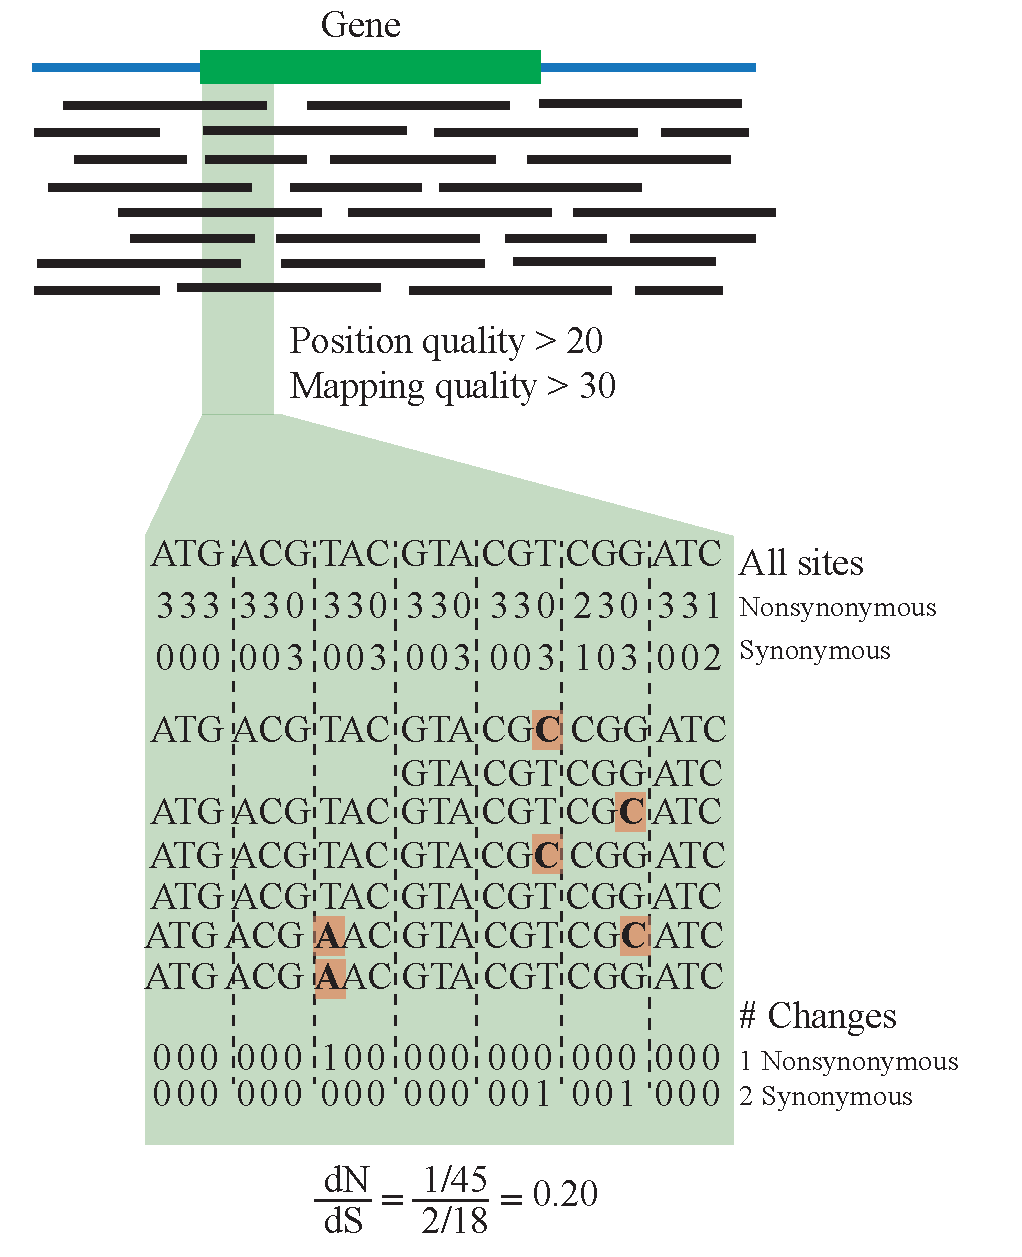
\includegraphics[width=\textwidth]{Chapter5/Figures/MappingStrategy.pdf}
  \caption{Mapping strategy}
  \label{MappingStrategy}
\end{figure}

%Table Genes positive selection
\begin{table}[hbt]
  \caption{Count of Genes under positive selection}
  \begin{tabularx}{\textwidth}{L{2.2cm}R{2cm}R{3cm}R{3.2cm}R{2cm}}
  \hline
    \textbf{Genome} & \textbf{CDS} & \textbf{January} & \textbf{August} & \textbf{Unique (Jan/Aug)} \\
    \hline
     \textit{J07HWQ1} & 3,584 & 568 (15.9) & 570 (15.9) & 4/6 \\
     \textit{J07HWQ2} & 3,856 & 565 (14.7) & 561 (14.6) & 6/2 \\
     \textit{J07HQX50} & 2,872 & 406 (14.1) & 405 (14.1) & 3/2 \\
     \textit{J07AB56} & 1,411 & 244 (17.3) & 236 (16.7) & 72/64 \\
     \textit{J07AB43} & 1,678 & 274 (16.3) & 281 (16.8) & 35/43 \\
     \textit{J07HN4} & 3,230 & 428 (13.3) & 427 (13.2) & 5/4 \\
     \textit{J07HN6} & 2,914 & 220 (7.6) & 218 (7.5) & 23/21 \\
     \textit{J07HX64} & 3049 & 603 (19.8) & 603 (19.8) & 3/3 \\
     \textit{J07HX5} & 2,139 & 374 (17.5) & 374 (17.5) & 2/2 \\
     \textit{J07HB67} & 2,847 & 494 (17.4) & 493 (17.3) & 60/59 \\
     \textit{J07HR59} & 1,841 & 145 (7.9) & 155 (8.4) & 3/13 \\
     \textit{A07HB70} & 2,514 & 479 (19.1) & 479 (19.1) & 6/6 \\
     \textit{A07HR67} & 2,891 & 507 (17.4) & 511 (17.7) & 0/4 \\
     \textit{A07HN63} & 2,507 & 212 (8.5) & 240 (9.6) & 9/37 \\
     \textit{A07HR60} & 2,861 & 375 (13.1) & 381 (13.3) & 10/16 \\
     \textit{G22} & 3,525 & 5 (0.14) & 5 (0.14) & 1/1 \\
     \textit{J07SB} & 1,641 & 290 (17.7) & 287 (17.5) & 6/3 \\     
  \end{tabularx}
  \label{PSgenes}
\end{table}


\todo{List of genes, product}
\todo{Functional categories, differences from the annotation?. Fisher test}
\todo{Plots of depth, dn/DS along genomes}

\section{Conclusions}

\section{Acknowledgments}

%%%%%%%%%%%%%%%%%%%%%%%


%\todo{Modify reference SNPs section}
%\subsection{Genome information and reference SNPs}
%To generate a list of reference SNPs,  11 archaeal genomes obtained from the assembly of the metagenomic samples were analyzed. The results (Table \ref{GenomeTable}), shows the total number of SNPs identified in each of the genomes. Although the low depth of the analysis does not allow to make any assumptions about the levels of genetic heterogeneity present on each population, still can provide a valid picture that can be contrasted with the Illumina data. Figure \ref{ReferenceSNPsType}, shows a comparison of the location and type of variation found among the genomes. Most of the identified polymorphisms are synonymous, meaning that they do not produce any changes in the amino acid sequence. Comparing among the populations, most of the polymorphisms fall into coding regions, with some extreme cases such as in \textit{Nanosalina} sp. J07AB43 and \textit{Nanosalinarum} sp. J07AB56, where only 5\% and 8\%, respectively, of the polymorpshism are found in intergenic regions. This reflects the streamlined nature of these genomes, and their reduced intergenic space \cite{Narasingarao:2012kp}. An interesting situation occurs in the case of \textit{Nanosalina} sp. J07AB43, which has a high number of polymorphisms classified as other (mostly frameshifts), close to a 51\%. This could be either result from assembly problems, or a reflection on the true genetic variability that is present in this population, but a higher level of resolution is needed to resolve this question.
%
%By looking at the annotation of each gene, we can begin to explore the possible functional effects of the found SNPs on each microbial population (Figure \ref{COG_TotalSNPs}). The averages values for each functional classification (Cellular Processes and Signaling: 19.1\%, Information Storage and Processing: 22.6\%, Metabolism: 39.9\% and Poorly characterized: 18.4\%), shows a higher percentage of SNPs (in average) in the metabolic functions. This can easily be explained by the larger number of genes that fall in this category. Even with this in mind, J07HQX50 shows a higher percentage of SNPs associated in the Cellular Processes and Signaling category, while J07AB43 and J07AB56 (members of the \textit{Nanohaloarchaea}) have a higher number of polymorphic sites in genes in the Information Storage and Processing and the Metabolic categories.
%
%Another important way to characterize the effects of the SNPs on each genomes is to look at the non-synonymous substitutions that are occurring across the genome, because the effect of this polymorphisms is to modify the resulting amino acid in the protein. The averages for each functional classification (Cellular Processes and Signaling: 18.1\%, Information Storage and Processing: 23.1\%, Metabolism: 38.5\% and Poorly characterized: 20.13\%), shows very similar values to the total count of SNPs (\ref{COG_NonSynSNPs}). Although the number of total and non-synonymous SNPs found in this part of the analysis is low to draw any conclusions about the effect on the overall microbial population, we observe that in the case of J07HR59 there are no non-synonymous polymorphisms associated with Cellular Processes and Signaling, while most fall in the Information category.
%
%To look more in detail at the effect of these non-synonymous SNPs, we can look more in detail at the functional classifications provided by COG. In the Cellular Processes and Signaling group, we can observe differences for the microbial populations (Figure \ref{ReferenceSNPs_NS_CellularProc}), which could be related to the low coverage observed for this reference SNPs, in particular in the case of J07HQX50, which has most of its SNPs associated with signal transduction mechanisms. Overall, the classification of these non-synonymous SNPs, shows that the majority falls in categories such as cell wall/membrane/envelope biogenesis, post-translational modifications and signal transduction mechanisms. These are functions that are related to the interaction of the organisms with the environments, such as phage infection and resistance mechanisms (REF), transporters (REF) and overall functions where it could be expected that changes in the amino acid sequences could be beneficial for the persistence of the microbial population in the environment. A similar situation can be observed in the case of the Information Storage and Processing category (Figure \ref{ReferenceSNPs_NS_Information}), where the more abundant in functions such as translation, ribosomal structure and biogenesis, and in proteins classified in the replication, recombination and repair group. Later in this chapter, we will explore the environmental adaptations of each microbial population, by using a deep-sequencing approach.
%
%In the case of functions that are part of the Metabolism group in the COG classification (Figure \ref{ReferenceSNPs_NS_Metabolism}), the trend is not as clear as in the other groups. The only two exceptions are J07HQX50 that has most of its polymorphisms associated with the inorganic ion transport and metabolism category, and J07HR59 that has most polymorphisms in the nucleotide transport and metabolism category. 
%
%Overall, this preliminary overview provides a set of expectetions on further analysis on the genetic heterogeneity of some of the microbial populaitons present in the Lake Tyrrell habitat. More important, by deconstructing the assembly of the Sanger reads, we can obtain a set of reference SNPs, which can be used for further population studies. This becomes very important consdiering that none of the organisms that were reocvered from the metagenoms is in culture, so targeting their genomes directly for SNP validation is not feasible, and other proxies need to be used. This dataset will be used for validation of the results of the mapping and variation detection in the following sections of this chapter.
%
%%TABLES
%
%\begin{table}[!htdp]
%\caption{Genome and reference SNPs}
%\begin{center}
%\resizebox{\textwidth}{!}{%
%\begin{tabularx}{\textwidth}{lp{2cm}p{2cm}p{3cm}}
%\hline
%%\textbf{Genome} & \textbf{Scaffold (JGI ID)} & \textbf{Length} & \textbf{SNPs} & \textbf{Change rate} \\
%\textbf{Genome}  & \textbf{Length} & \textbf{SNPs} & \textbf{Change rate} \\
%
%\hline \hline
%\multirow{2}{*}{\textit{Halonotius} sp. J07HN4} & 547,037 & 963 & 568\\
%& 2,341,623 & 7,985 & 293 \\
%\hline
%
%\multirow{6}{*}{\textit{Halonotius} sp. J07HN6} & 61,036 & 603 & 101 \\
% & 89,290 & 558 & 160 \\
% & 185,112 & 1,482 & 124 \\
% & 424,200 & 2,761 & 153 \\
% & 873,166 & 6,463 & 135 \\
%& 896,196 & 5,455 & 164 \\
%\hline
%
%uncultured archaeon sp. J07HX64 & 2,982,938 & 5,468 & 545 \\
%\hline
%\multirow{3}{*}{\textit{Halobaculum} sp. J07HB67} & 110,024 & 62 & 1,744 \\
%& 254,249 & 145 & 1,753 \\
%& 2,285,274 & 2,855 & 800 \\
%\hline
%
%\multirow{2}{*}{\textit{Haloquadratum} sp. J07HQX50} & 1,543,888 & 28 & 55,138 \\
%& 1,476,021 & 131 & 11,267 \\
%\hline
%
%\multirow{4}{*}{\textit{Halorubrum} sp. J07HR59} & 72,446 & 1 & 72,466 \\
%& 49,857 & 29 & 1,719 \\
%& 184,023 & 7 & 26,289 \\
%& 1,672,266 & 255 & 6,557 \\
%\hline
%
%\textit{Haloquadratum walsbyi} J07HQW1 & 3,475,501 & 24,743 & 140 \\
%\hline
%
%\textit{Haloquadratum walsbyi} J07HQW2 & 3,594,539 & 13,897 & 258 \\
%\hline
%
%uncultured archaeon J07HX5 & 2,040,945 & 2,047 & 997 \\
%\hline
%
%\multirow{7}{*}{\textit{Nanosalina} sp. J07AB43} & 54,503 & 295 & 184 \\
%& 111,825 & 1,037 & 107 \\
%& 65,032 & 876 & 74 \\
%& 32,088 & 304 & 105 \\
%& 112,863 & 2,296 & 49 \\
%& 52,428 & 1,288 & 40 \\
%& 798,418 & 11,578 & 68 \\
%\hline
%
%\multirow{3}{*}{\textit{Nanosalinarum} sp. J07AB56} & 195,424 & 1,540 & 127 \\
%& 60,285 & 196 & 307 \\
%& 959,093 & 6,837 & 140 \\
%\hline
%
%
%\end{tabularx}
%}
%\end{center}
%\label{GenomeTable}
%\end{table}
%
%
%%FIGURES
%
%\begin{figure}[!htbp]
%	\centering
%	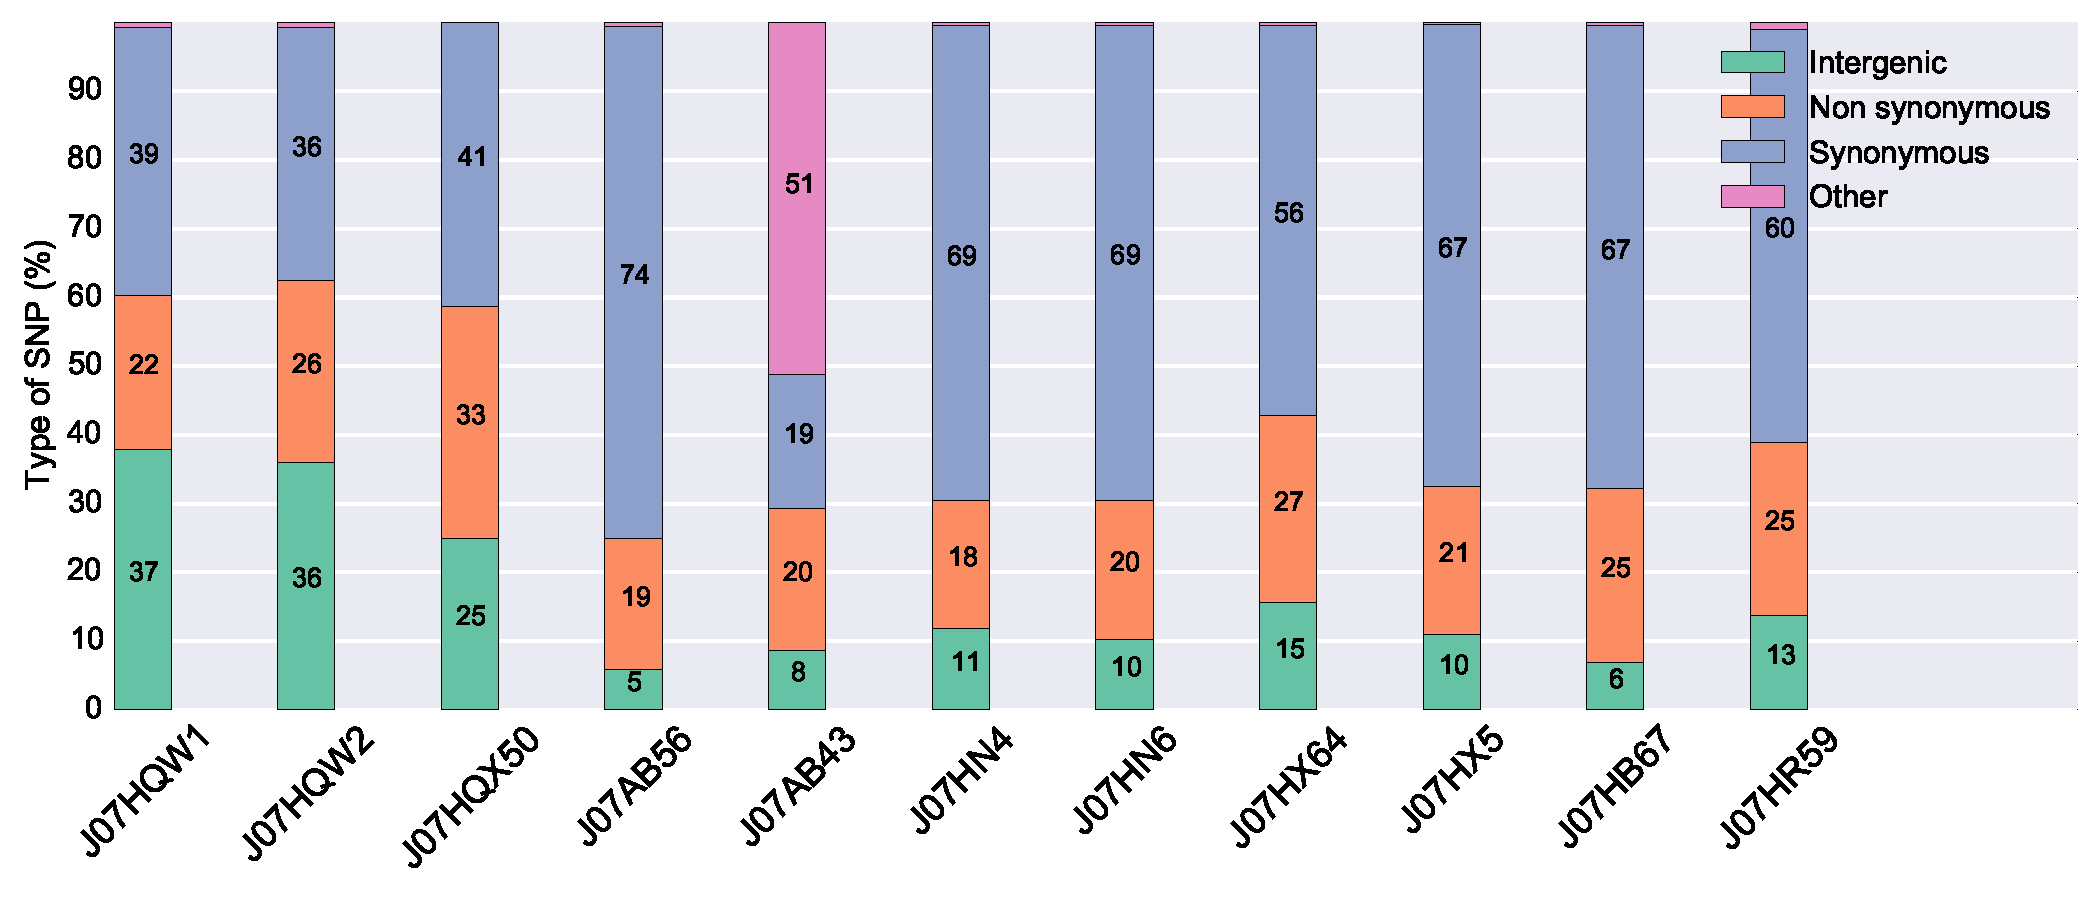
\includegraphics[width=\textwidth]{Chapter5/Figures/ReferenceSNPtypes.pdf}
%	\caption{Classification of the reference SNPs, by type.}
%	\label{ReferenceSNPsType}
%\end{figure}
%
%%FIGURE
%\begin{figure}[!htbp]
%	\centering
%	\subfloat[Total SNPs \label{COG_TotalSNPs}]{%
%		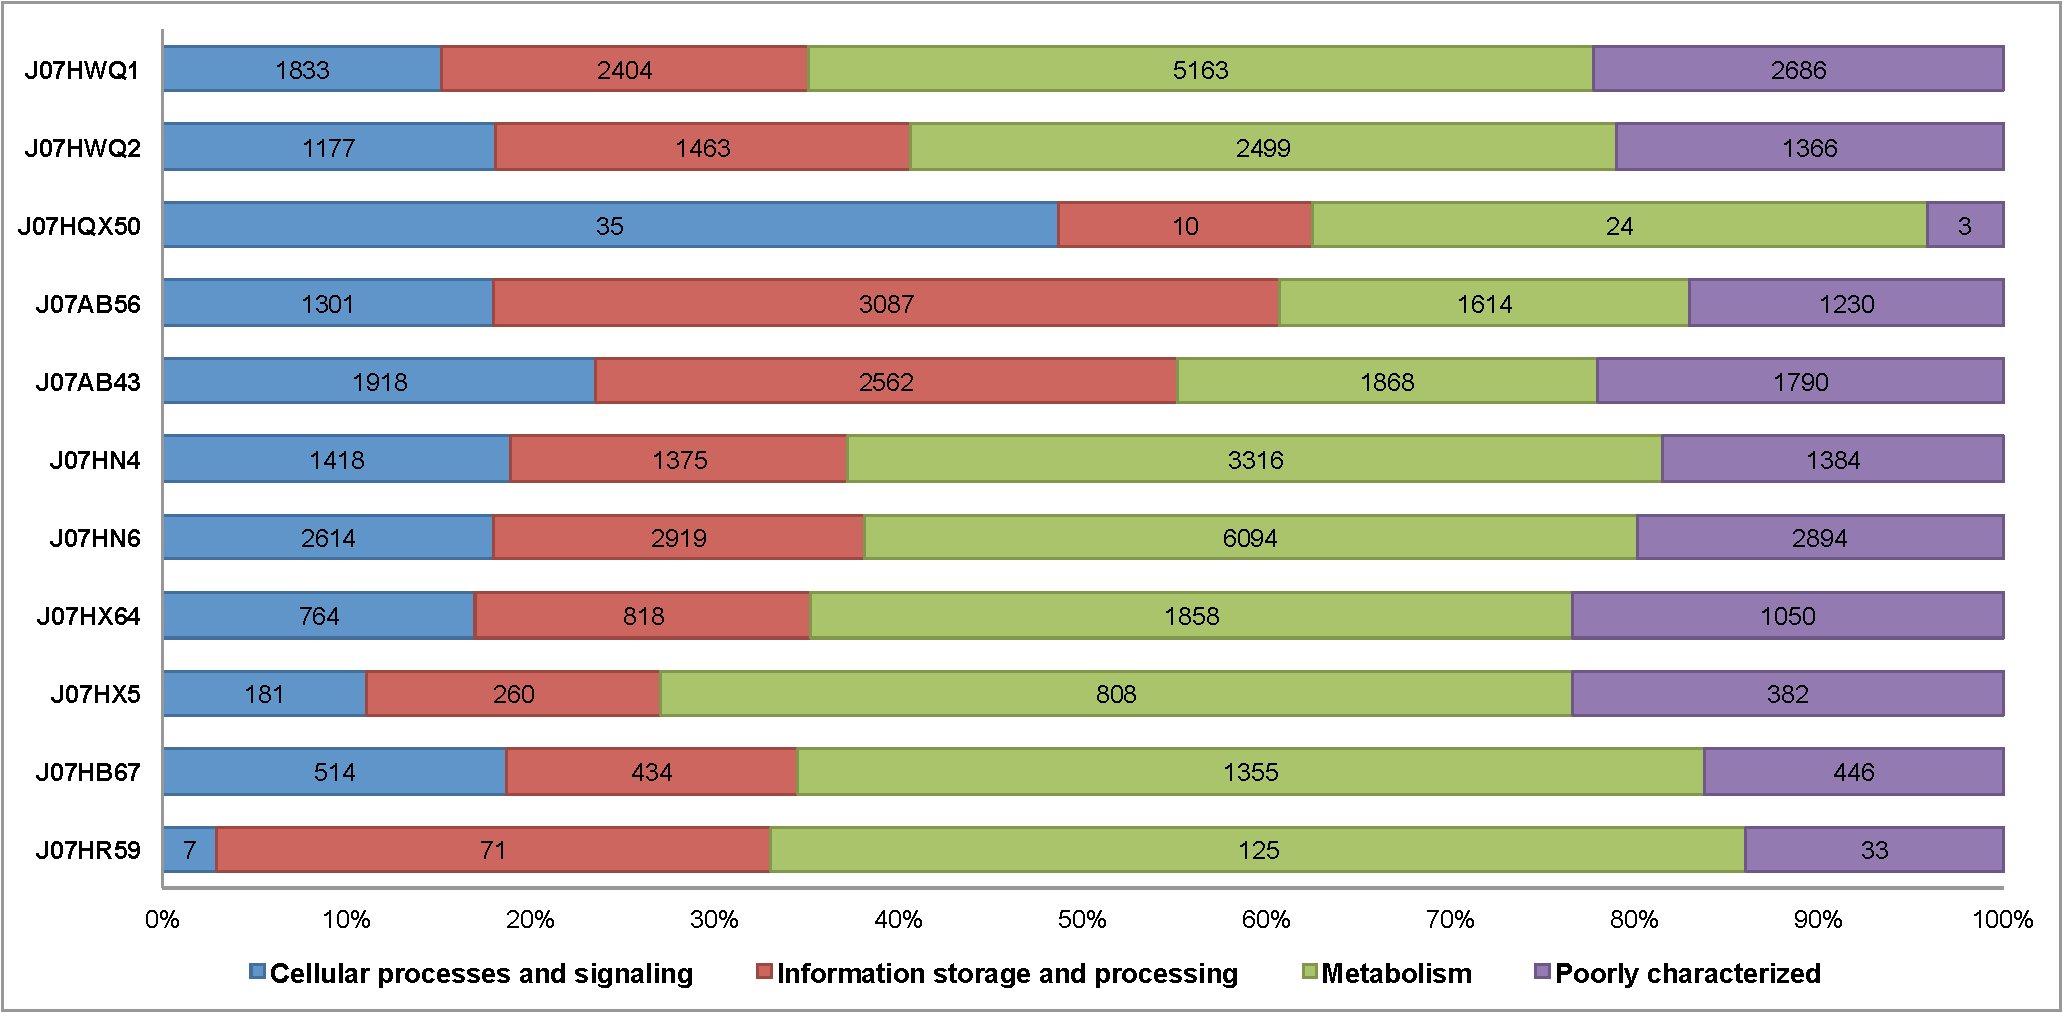
\includegraphics[width=\textwidth]{Chapter5/Figures/ReferenceSNPs_COGsTotal.pdf}
%	}
%	\hfill
%	\subfloat[Non-synonymous SNPs\label{COG_NonSynSNPs}]{%
%		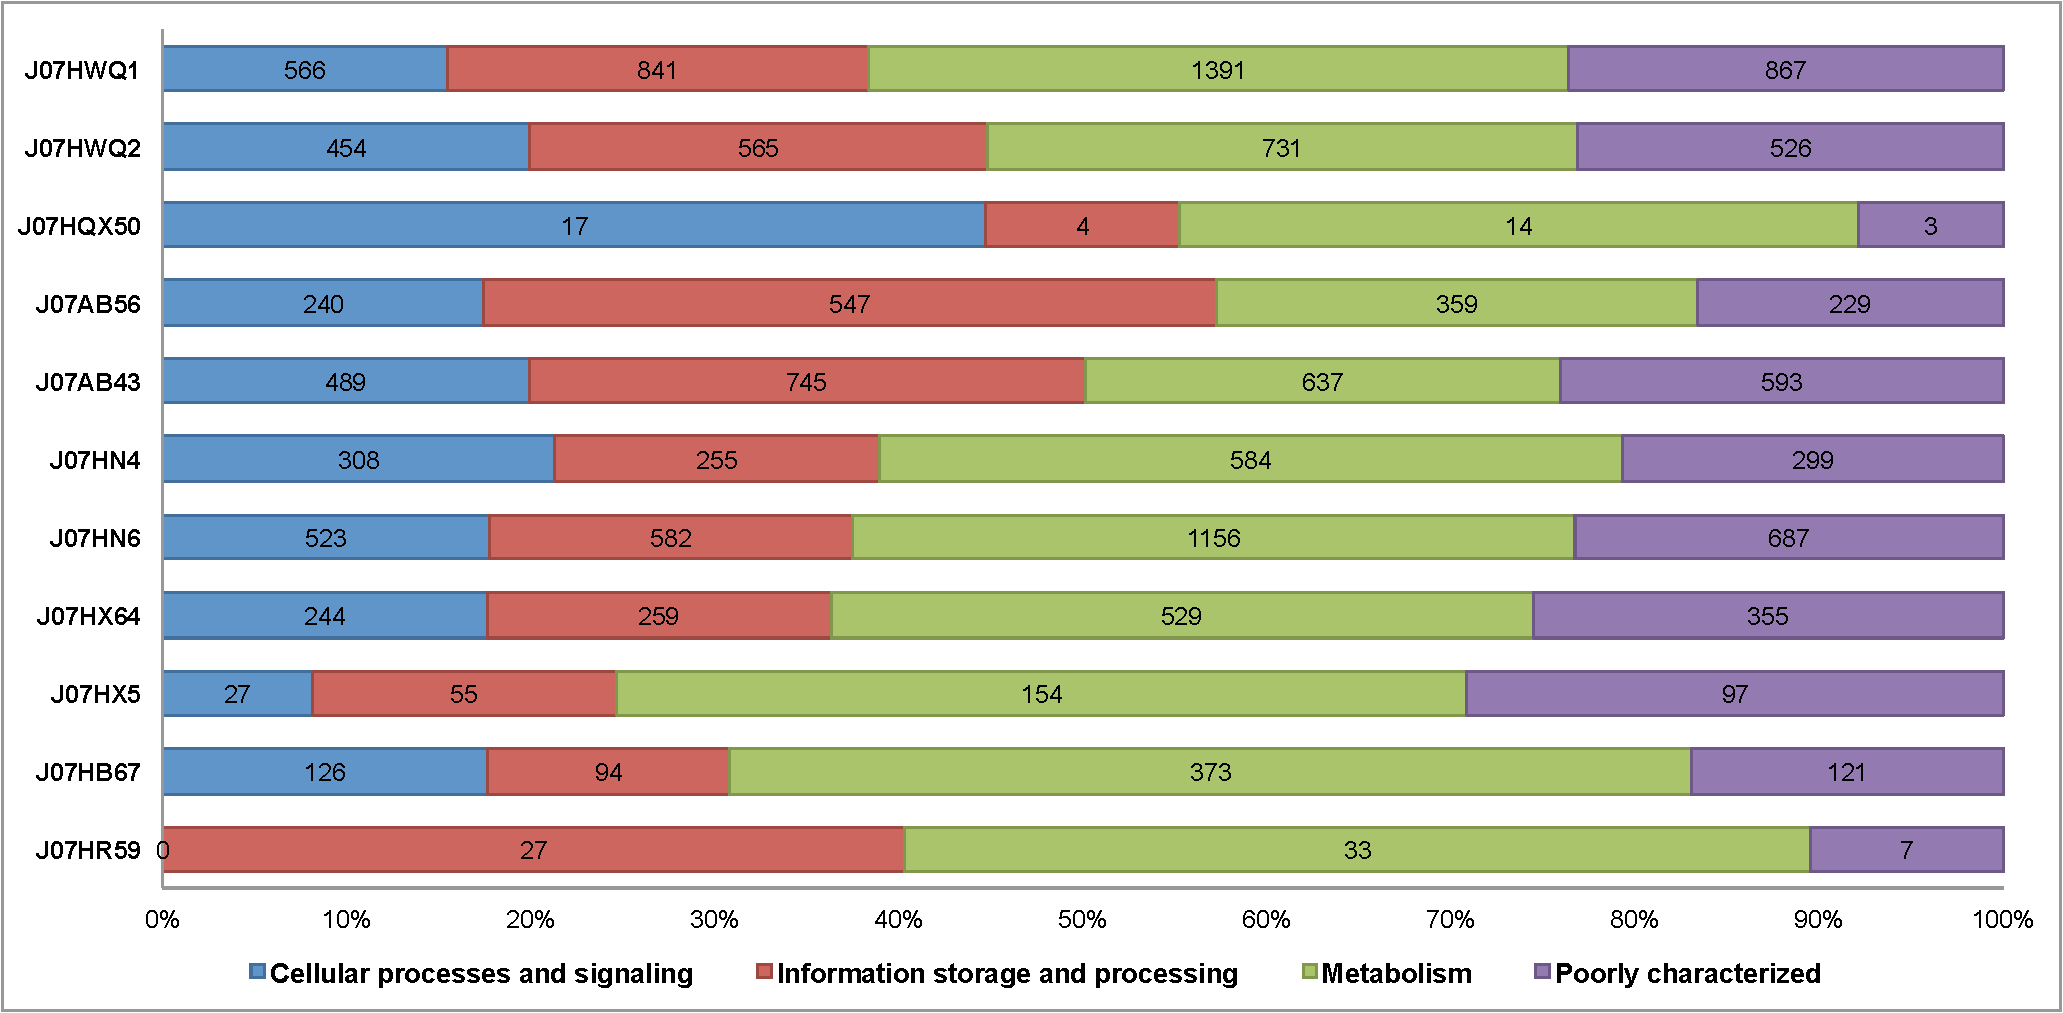
\includegraphics[width=\textwidth]{Chapter5/Figures/ReferenceSNPs_COGs_NS.pdf}
%	}		
%	\caption{Comparison between the total number and the non-synonymous SNPs found in each genome, associated to functional categories from the COG classification }
%	\label{ReferenceSNPs_COGsSummary}
%\end{figure}
%
%%FIGURE
%
%\begin{figure}[!htbp]
%	\centering
%	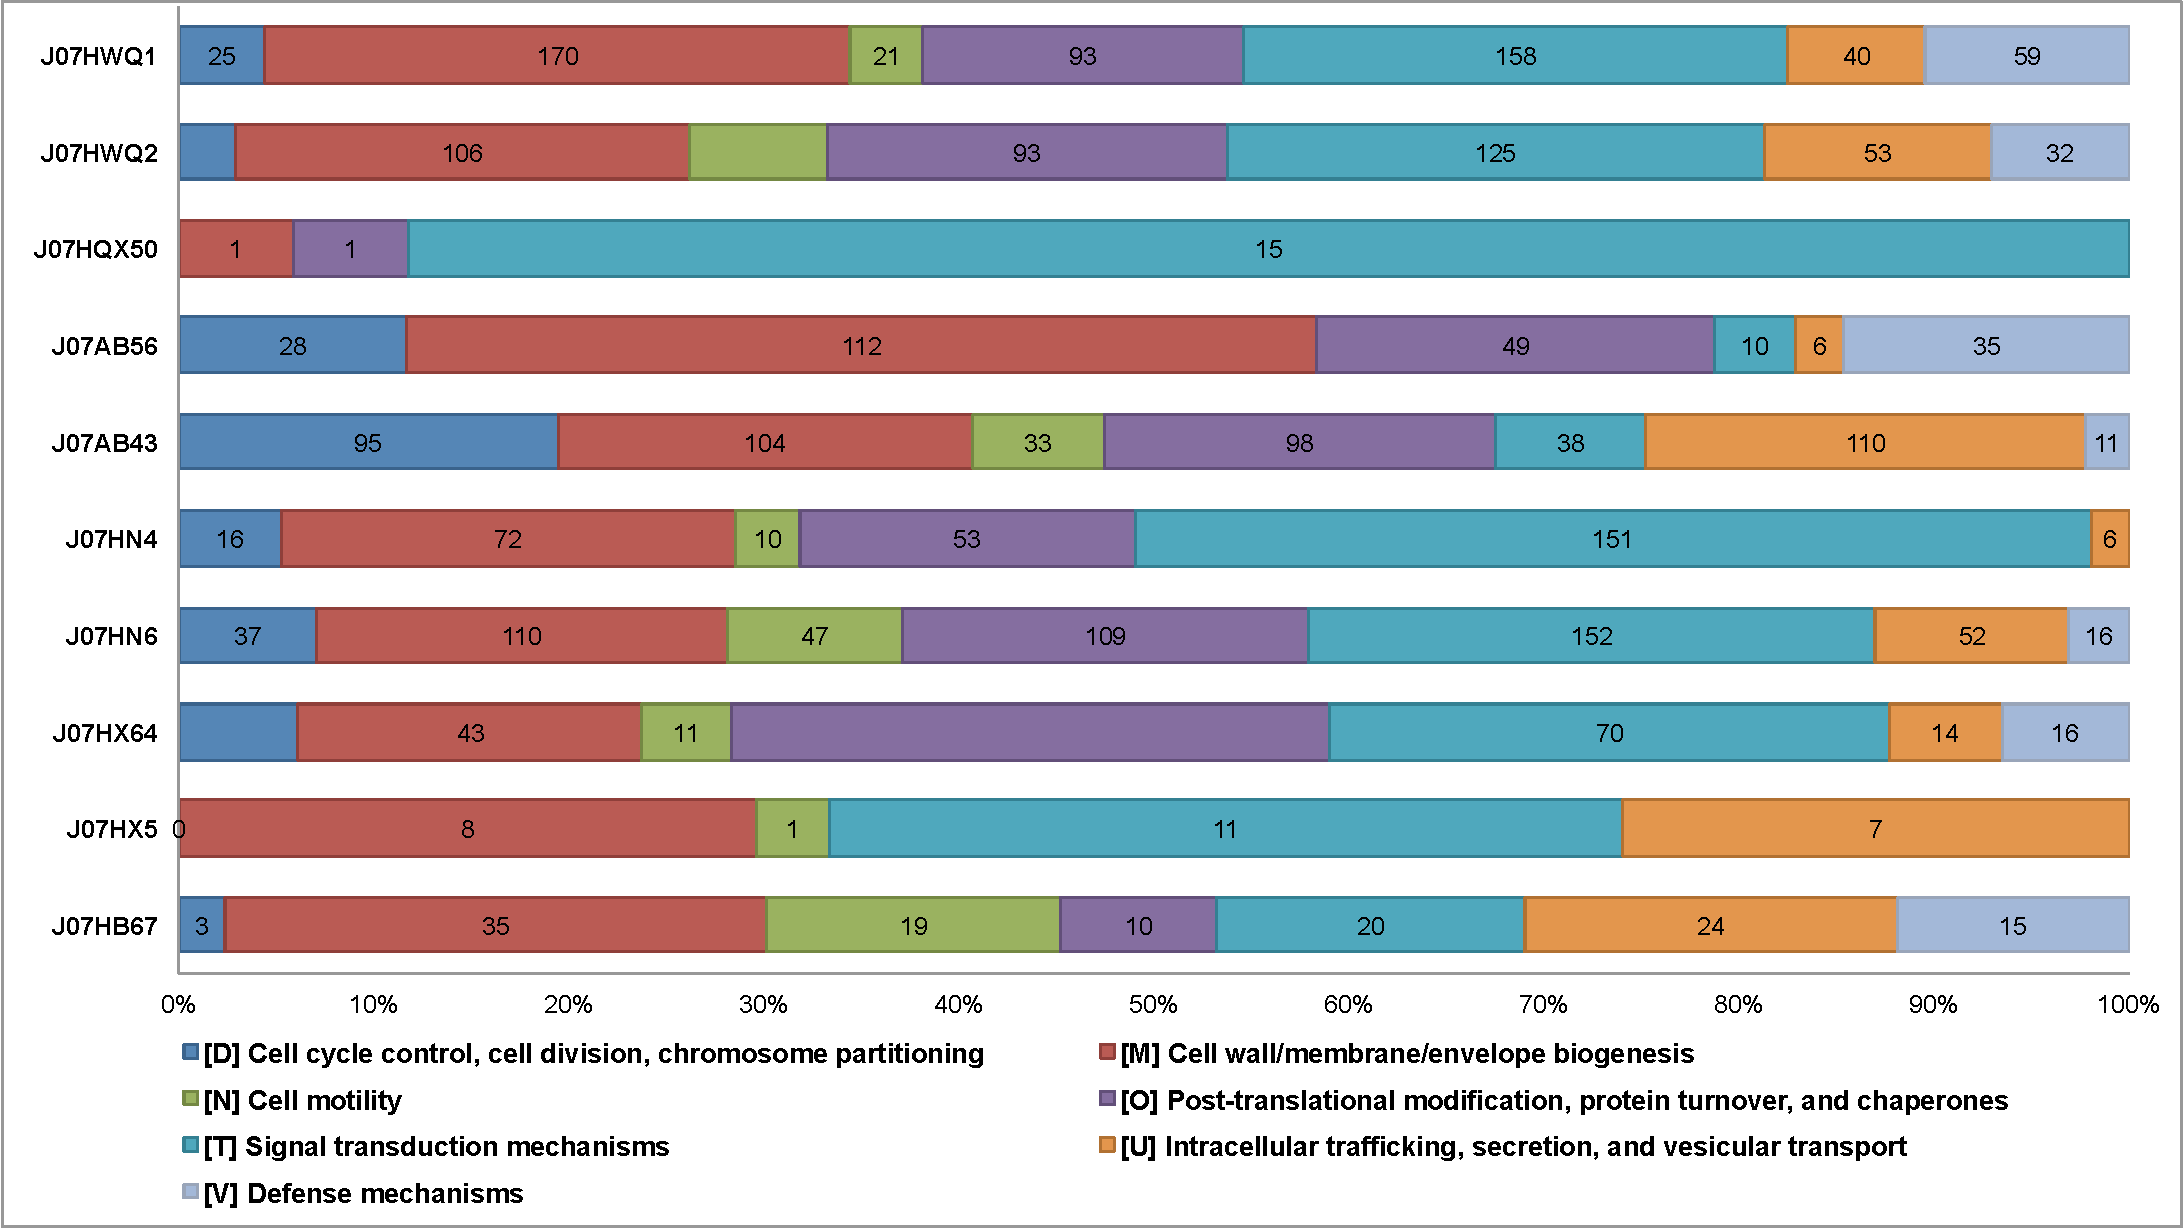
\includegraphics[width=\textwidth]{Chapter5/Figures/ReferenceSNPs_NonSyn_CellularProc.pdf}
%	\caption{Count of non-synonymous SNPs found in COGs categories from the Cellular Processes and Signaling group}
%	\label{ReferenceSNPs_NS_CellularProc}
%\end{figure}
%
%\begin{figure}[!htbp]
%	\centering
%	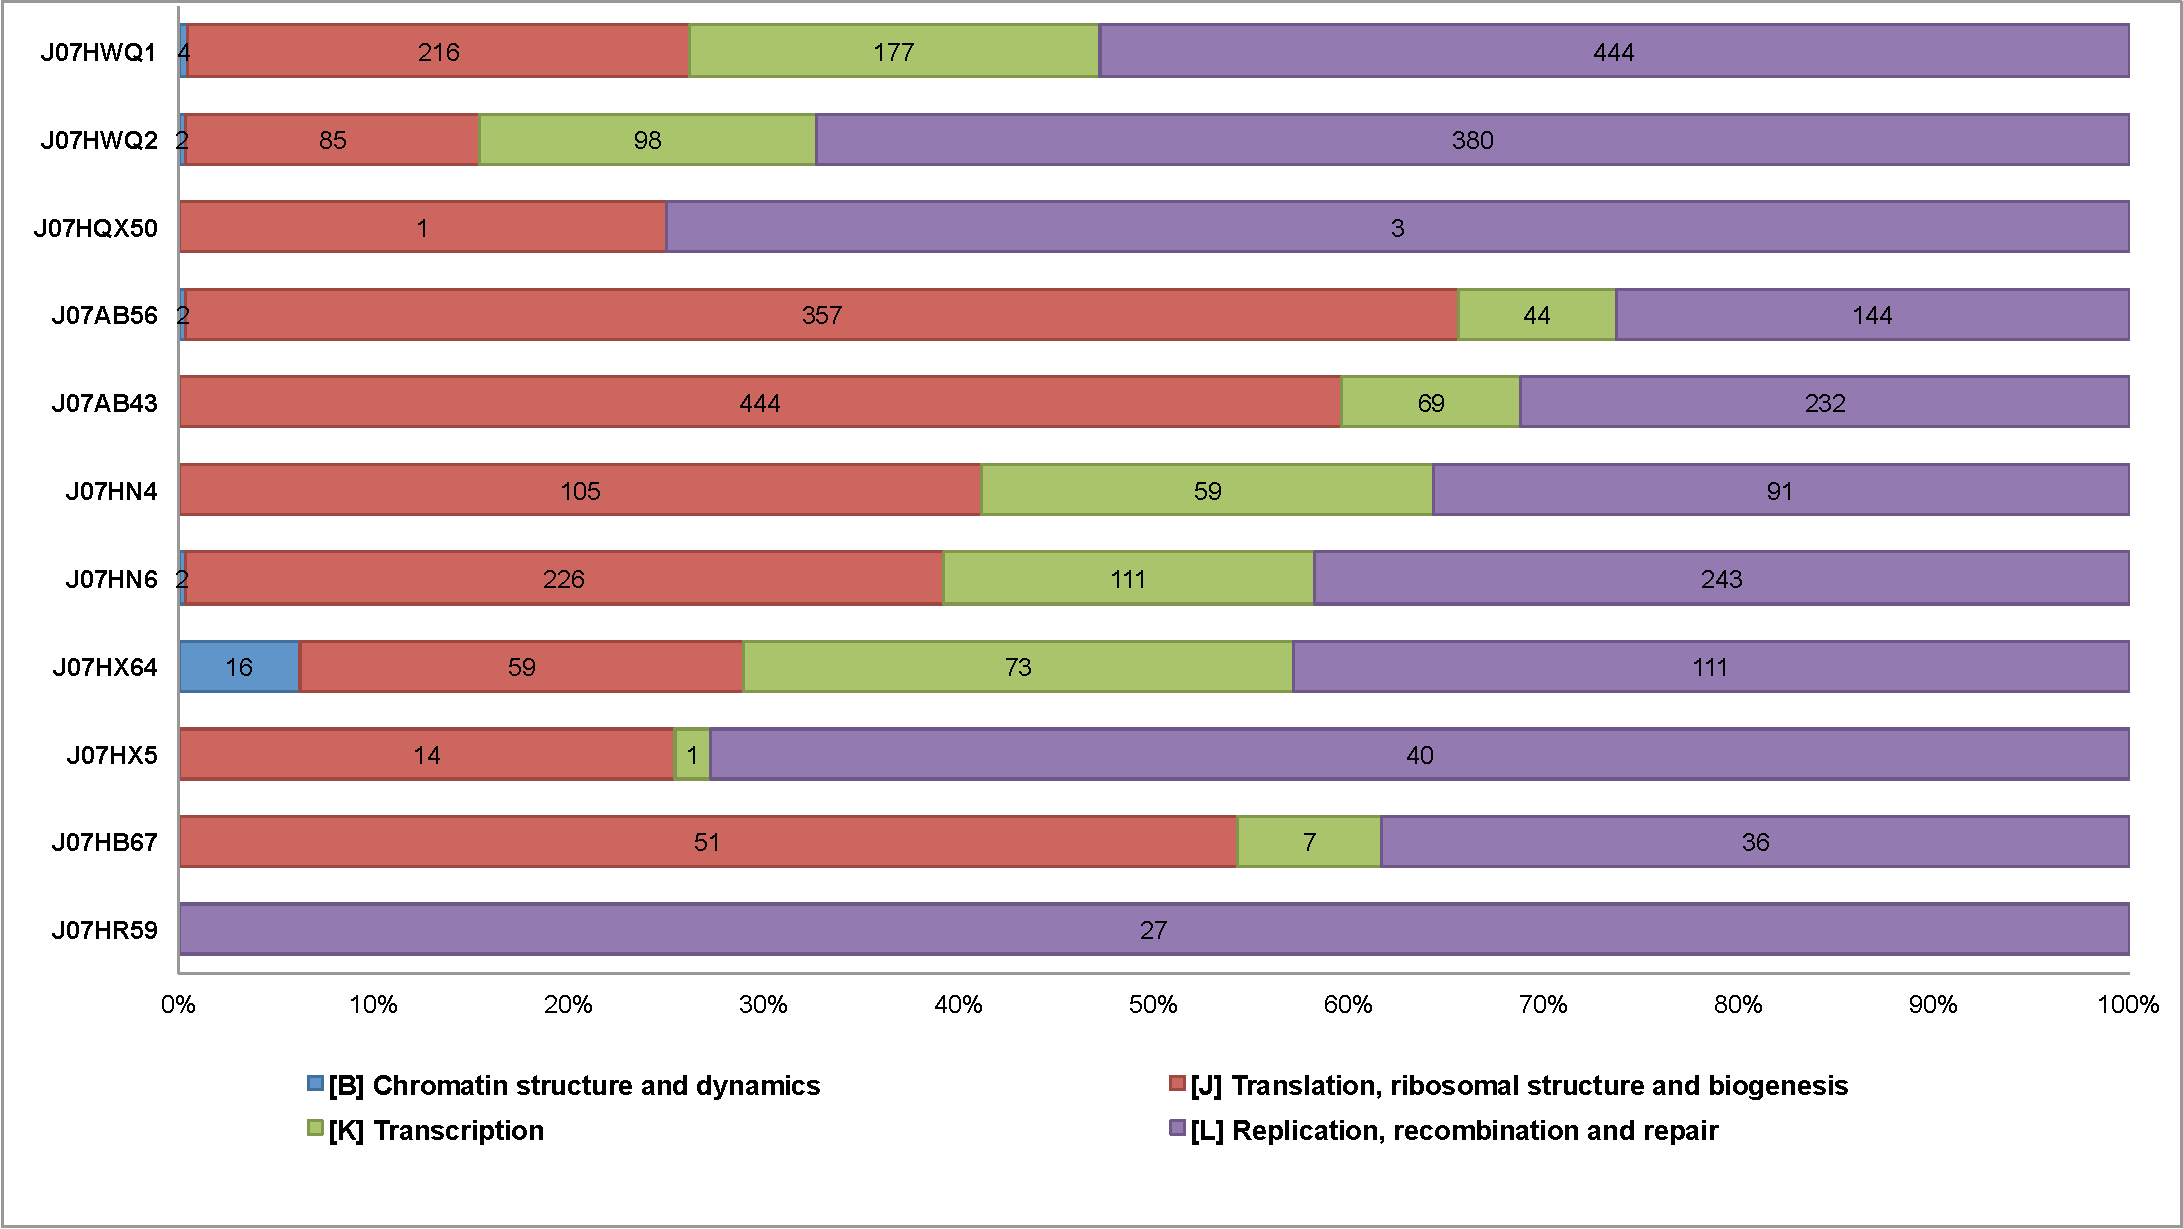
\includegraphics[width=\textwidth]{Chapter5/Figures/ReferenceSNPs_NonSyn_Information.pdf}
%	\caption{Count of non-synonymous SNPs found in COGs categories from the Information Storage and Processing group}
%	\label{ReferenceSNPs_NS_Information}
%\end{figure}
%
%\begin{figure}[!htbp]
%	\centering
%	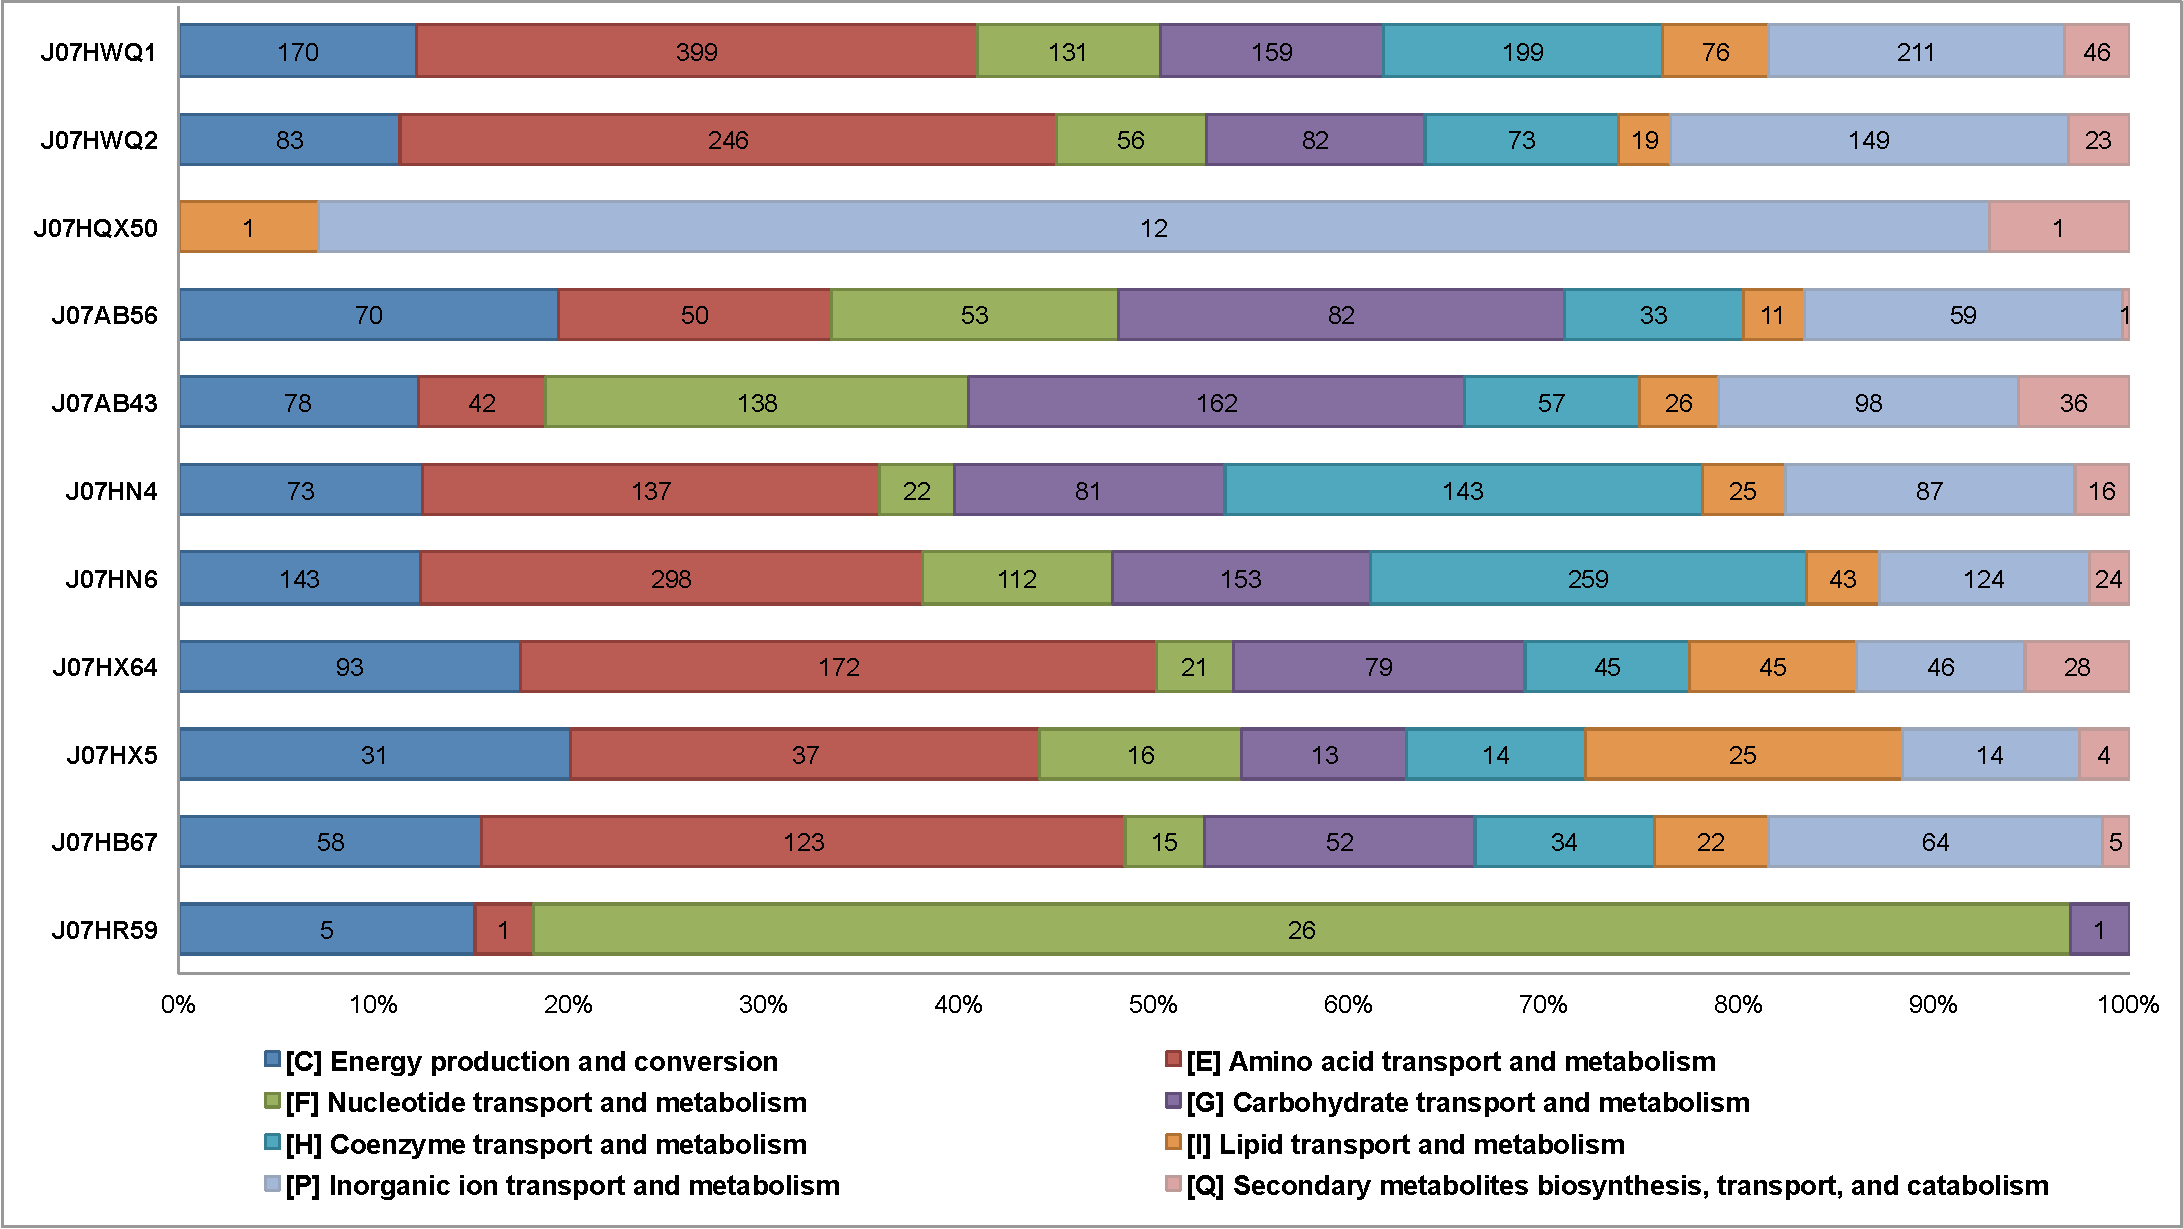
\includegraphics[width=\textwidth]{Chapter5/Figures/ReferenceSNPs_NonSyn_Metabolism.pdf}
%	\caption{Count of non-synonymous SNPs found in COGs categories from the Metabolism group}
%	\label{ReferenceSNPs_NS_Metabolism}
%\end{figure}
%
%
%

%\subsection{Selection analysis of the reference SNPs}
%- Genes found under positive selection
%- Functional differences of the genes under positive selection
%- Categories, etc

%
%
%Comparison between assembly and read mapping
%
%The comparison between the number of reads used in the assembly of the archaeal populations, versus mapping the reads back to these genomes, indicates that only a low percentage of the reads were not recovered by mapping (XX\%) (Figure X). In addition, mapping of the reads allows the recovery of reads that were not incorporated into the assemblies.
%
%Even when the number the depth of coverage is increase when the reads are mapped back to the reference genomes (Table X), the overall distribution of depths along the genome shows a similar trend (Figure X), indicating that even with that more reads are recruited (increasing the depth of coverage and posiblly the number of SNPS presents compared to an assembly-based analysis), we are not overrepreseting areas of the genome.
%
%We observed differences when looking at the coverage of individual genes, where a small percentage in each genome (XX, Table X) showed less coverage than expected. Neverhelss, this is only a small fraction of the total number of genes present (Figure X).
%
%Look at the gene with transport, secretory or motilify functions in detail. Look a the dN/dS ratiosn in a sliding window (201 bp?)
%
%For hypothetica proteins, look at SCOP classification
%


%
%\begin{figure}[htbp]
%	\centering
%	*
%	\caption{Analysis pipeline workflow}
%	\label{WorkflowAnalysisSNPs}
%\end{figure}
%
%
%\begin{figure}[htbp]
%	\centering
%	*
%	\caption{Mapped reads per genome}
%	\label{ReadMappingGenomes}
%\end{figure}
%
%\begin{figure}[htbp]
%	\centering
%	*
%	\caption{Depth of coverage for each genome}
%	\label{DepthCoverageGenomes}
%\end{figure}
%
%\begin{figure}[htbp]
%	\centering
%	*
%	\caption{SNPs in COGs}
%	\label{COGsSNPs}
%\end{figure}
%
%\begin{figure}[htbp]
%	\centering
%	*
%	\caption{Transition transversion rates}
%	\label{TTrates}
%\end{figure}
%
%\begin{figure}[htbp]
%	\centering
%	*
%	\caption{Network diagram SNPs}
%	\label{NetworkSNPs}
%\end{figure}
%
%\begin{figure}[htbp]
%	\centering
%	*
%	\caption{Map of SNPs in contigs}
%	\label{SNPsContigMap}
%\end{figure}
%
%\begin{figure}[htbp]
%	\centering
%	*
%	\caption{SNP rarefaction curve per population}
%	\label{SNPsRarefaction}
%\end{figure}
%
%\begin{figure}[htbp]
%	\centering
%	*
%	\caption{Calculation of pN/pS ratios}
%	\label{pNpS_diagram}
%\end{figure}
%
%\begin{figure}[htbp]
%	\centering
%	*
%	\caption{Histogram of dN/dS ratios}
%	\label{pNpS_hist}
%\end{figure}



%\bibliographystyle{abbrv}
%\bibliography{CompleteLibrary}